% ================================================================
%  TokenMizer: Graph-Structured Session Memory for
%  Long-Horizon LLM Context Management
%  IEEE Transactions Style — Journal Version
%  Single benchmark (21 sessions). All values measured.
%  No estimated results. Full statistical reporting.
% ================================================================
\documentclass[journal]{IEEEtran}

\usepackage{amsmath,amssymb,amsthm}
\usepackage{graphicx}
\usepackage{booktabs}
\usepackage{array}
\usepackage{colortbl}
\usepackage{xcolor}
\usepackage{url}
\usepackage{balance}
\usepackage{multirow}
\usepackage{algorithm}
\usepackage{algorithmic}
\usepackage[colorlinks=true,
            linkcolor=blue!60!black,
            citecolor=blue!60!black,
            urlcolor=blue!60!black]{hyperref}

\definecolor{rowours}{HTML}{FEF9C3}
\definecolor{rowgood}{HTML}{DCFCE7}

\newtheorem{definition}{Definition}
\newtheorem{proposition}{Proposition}

\tolerance=9999
\emergencystretch=4em
\hbadness=10000

% ================================================================
\title{TokenMizer: Graph-Structured Session Memory\\
for Long-Horizon LLM Context Management}

\author{Shweta~Mishra%
\thanks{Independent Researcher, India.
E-mail: \href{mailto:shweta.mishra.research@gmail.com}{shweta.mishra.research@gmail.com}.
Code and benchmark: \url{https://github.com/Shweta-Mishra-ai/tokenmizer}.
Manuscript received June 4, 2026.}%
}

% ================================================================
\begin{document}
\maketitle

% ================================================================
\begin{abstract}
Large language model (LLM) deployments for long-horizon tasks
face a fundamental constraint: context windows are finite while
productive work sessions are not.
When session history exceeds the Maximum Effective Context
Window (MECW), critical structured information---architectural
decisions, task status transitions, file modification histories,
and resolved errors---is silently discarded.
Existing mitigations (truncation, summarization, retrieval
augmentation) treat history as flat text, destroying the
typed, relational structure that makes sessions resumable.

We present \textbf{TokenMizer}, an open-source proxy system
that models LLM session history as a typed knowledge graph.
The graph schema defines \textbf{14 node types} with status
lifecycles and \textbf{7 semantic edge types}.
A hybrid extraction pipeline (heuristic with LLM upgrade path)
populates the graph incrementally.
A three-tier checkpoint system serializes the graph into
compact, structured resume blocks.
An 8-layer compression pipeline reduces context overhead, and
a sentence-embedding semantic cache reduces repeated-query
latency.

We evaluate TokenMizer on a controlled benchmark of
\textbf{21 sessions spanning 5 application domains} (software
engineering, data science, DevOps, research/writing, and
debugging) with manually annotated ground truth.
\textit{All reported results are measured on this benchmark;
no estimated values are presented.}
The benchmark is a synthetic but carefully constructed
corpus; evaluation on live developer sessions is identified
as the highest-priority future work.

The primary result is token economy: TokenMizer produces
resume blocks averaging \textbf{78 tokens}
($\sigma\!=\!21.4$, range: 42--124)---\textbf{$2\times$
smaller than any evaluated baseline} (159--170 tokens)---while
achieving \textbf{higher decision recall than all three
baselines} (+9--17~percentage points).
Decision recall is the key structural metric: no evaluated
baseline preserves \emph{why} a technology was chosen,
only that it was mentioned.

Across 21 sessions and 5 domains, TokenMizer achieves mean
task recall $51.0\%$ ($\sigma\!=\!32.7\%$), decision recall
$46.6\%$ ($\sigma\!=\!32.0\%$), and file recall $58.7\%$
($\sigma\!=\!46.7\%$).
High variance reflects genuine domain heterogeneity: sessions
with explicit imperative phrasing (software engineering) score
substantially higher than sessions with implicit reasoning
(research, planning).
This distinction is addressed in the Limitations section.

Ablation studies establish that fuzzy label matching
contributes $+33$~percentage points of task recall
improvement---the dominant single improvement factor.
The heuristic compression pipeline achieves \textbf{47.3\%}
token reduction without external dependencies.
A novel \textbf{token efficiency} metric---recall per
100 resume tokens---reveals debugging sessions as the
highest-efficiency domain (mean $\eta\!=\!0.91$).

TokenMizer is released as open-source software (MIT licence)
at \url{https://github.com/Shweta-Mishra-ai/tokenmizer}.
\end{abstract}

\begin{IEEEkeywords}
large language models, context management, session memory,
knowledge graph, prompt compression, semantic caching,
long-horizon tasks, developer tools, information extraction
\end{IEEEkeywords}

% ================================================================
\section{Introduction}
\label{sec:intro}
% ================================================================

\IEEEPARstart{L}{arge} language model (LLM) deployments for
software engineering~\cite{sweagent,copilot}, data
science~\cite{housurvey}, and research assistance increasingly
involve \emph{long-horizon sessions}: multi-turn interactions
spanning hours, where each turn builds on the accumulated
context of previous turns.
These sessions develop rich internal structure: technology
choices made in turn 3 constrain implementation options in
turn 12; errors resolved in turn 7 inform test strategies in
turn 15; files modified in turn 4 must be updated consistently
in turn 18.

The fundamental constraint is context window capacity.
Paulsen~\cite{paulsen2025} defines the \emph{Maximum Effective
Context Window} (MECW) as the context length at which model
task accuracy degrades below an acceptable threshold.
Critically, MECW is substantially lower than the advertised
maximum context window (MCW) for complex, multi-step tasks.
Liu et al.~\cite{lostmiddle} further demonstrate that content
placed in the \emph{middle} of long contexts is systematically
under-attended, amplifying the effective degradation.
At approximately 950~tokens per turn, a development session
exhausts a 16{,}000-token MECW after only 16~turns.

\subsection{Limitations of Existing Approaches}

Three categories of mitigation exist, each with a structural
limitation.

\textbf{Truncation-based methods}~\cite{brownfewshot} discard
the oldest messages when the context budget fills.
This preserves recency but discards exactly the content
that matters most: architectural decisions, initial technology
choices, and goal definitions established early in a session.

\textbf{Summarization-based methods}~\cite{langchain,acc}
produce free-text summaries via a secondary LLM call.
These compress well but are structurally imprecise: a natural
language summary cannot reliably distinguish a \emph{completed}
task from a \emph{pending} one, nor can it preserve the
\emph{rationale} for a technology decision.
The summary of ``We decided to use Redis for session storage
because it supports TTL natively'' and ``We considered Redis
but chose PostgreSQL'' may be informationally indistinguishable.

\textbf{Retrieval-augmented methods}~\cite{rag,memgpt}
retrieve relevant passages on demand using vector similarity.
These may miss contextually relevant but semantically distant
information: an early environment decision may be critical to
a late deployment question yet fail to retrieve because the
embedding distance between the two turns is large.

A key distinction between TokenMizer and MemGPT~\cite{memgpt}
is scope. MemGPT targets long-term factual recall
\emph{across} sessions using an OS-inspired hierarchical
memory model controlled by the LLM itself. TokenMizer targets
per-session structural continuity through a transparent
proxy requiring zero application-level changes.
Both approaches address different failure modes of the same
underlying constraint.

\subsection{Key Insight and Contributions}

The core insight motivating TokenMizer is that
\textbf{session history is not flat text---it is a structured
knowledge artifact}. Every developer session contains:
\begin{itemize}
  \item \emph{Tasks} with explicit status lifecycles
    (pending $\to$ in-progress $\to$ completed/failed);
  \item \emph{Decisions} with rationales that constrain future
    choices;
  \item \emph{Files} whose modification history defines the
    codebase state;
  \item \emph{Errors} and their resolutions;
  \item \emph{Environment} facts (runtime versions,
    infrastructure choices) that scope all other nodes.
\end{itemize}
These entities are connected by typed relationships
(\textsc{implements}, \textsc{fixes}, \textsc{depends-on},
etc.) that encode causal and structural dependencies.

A representation that preserves this \emph{structure} enables
efficient, queryable context preservation: discard the raw
conversation tokens; retain the typed graph; serialize to a
compact resume block.
The structural encoding also enables a qualitatively different
kind of recall: knowing that a decision node encodes a
technology choice with its rationale is not equivalent to
knowing that the word ``Redis'' appears somewhere in retained
text.

\textbf{Contributions:}
\begin{enumerate}
\item A \textbf{formal typed knowledge graph schema} for LLM
  sessions with 14 node types, 7 edge types, and a
  well-defined status transition system
  (Section~\ref{sec:graph}).
\item A \textbf{hybrid extraction pipeline} with V1/V2
  heuristic and LLM upgrade path, with a full
  \textbf{ablation study} identifying the contribution of
  each improvement (Section~\ref{sec:extraction}).
\item A \textbf{three-tier checkpoint system} with graph diffs
  and token-budgeted serialization
  (Section~\ref{sec:checkpoint}).
\item An \textbf{8-layer heuristic compression pipeline}
  achieving 47.3\% token reduction at zero inference cost,
  with optional neural stages (Section~\ref{sec:compression}).
\item A \textbf{semantic embedding cache} with measured
  hit rate on a controlled repeated-query workload
  (Section~\ref{sec:cache}).
\item A \textbf{21-session benchmark} spanning 5 domains
  with ground-truth annotations and a novel
  \textbf{token efficiency metric}, released publicly
  (Section~\ref{sec:experiments}).
\item A \textbf{correlation analysis} of session properties
  with extraction quality, yielding actionable design
  implications (Section~\ref{sec:analysis}).
\end{enumerate}

% ================================================================
\section{Background and Related Work}
\label{sec:related}
% ================================================================

\subsection{Context Window Degradation}

Paulsen~\cite{paulsen2025} introduces the MECW concept,
demonstrating empirically that all tested frontier models
degrade in accuracy on multi-step tasks before reaching
their advertised MCW.
For a model with MCW\,=\,128{,}000 tokens, the MECW may be
as low as 16{,}000 tokens for complex coding tasks.
This motivates the 16k-token MECW used as the running example
throughout this paper.

Liu et al.~\cite{lostmiddle} demonstrate the ``lost in the
middle'' phenomenon: retrieval and multi-document QA tasks
show U-shaped accuracy profiles, with content in the middle
of long prompts systematically under-used.
This amplifies the effective degradation: even content that
nominally fits within MCW may not be reliably attended.

\subsection{Memory Systems for LLMs}

\textbf{MemGPT}~\cite{memgpt} proposes an OS-inspired
hierarchical memory model distinguishing main context (fast,
limited) from external storage (slow, unlimited).
Memory management is explicit, controlled by the LLM itself,
with paging operations inserted as function calls.
MemGPT targets long-term factual recall across sessions;
TokenMizer targets per-session structural continuity at
zero inference cost.

\textbf{LangChain Memory}~\cite{langchain} provides several
memory backends including ConversationKGMemory, which is
architecturally most similar to TokenMizer.
The key differences are: LangChain's KG memory uses an
untyped, schema-free graph; extraction quality and node
lifecycle management are developer responsibilities; and the
backend requires explicit integration rather than a
transparent proxy.
TokenMizer provides a formal schema with 14 typed node
classes, status lifecycle enforcement, and a validation layer.

\textbf{Active Context Compression (ACC)}~\cite{acc} compresses
context by autonomous LLM calls, achieving 22.7\%
in-session compression.
TokenMizer's heuristic pipeline achieves 47.3\% without any
inference calls, making it substantially more efficient
before neural stages are applied.
The tradeoff is coverage: LLM-based extraction addresses
implicit phrasing that heuristics cannot reach.

\subsection{Prompt Compression}

\textbf{LLMLingua}~\cite{llmlingua} and
\textbf{LongLLMLingua}~\cite{longllmlingua} use small proxy
LLMs to compute per-token importance scores, removing
low-importance tokens at 2--6$\times$ compression ratios.
TokenMizer incorporates LLMLingua-2 as layers 7--8 in its
compression pipeline, applied after heuristic preprocessing
has removed structurally trivial content.

\textbf{RECOMP}~\cite{recomp} applies selective summarization
for retrieval-augmented generation (RAG), retrieving only
relevant passages.
TokenMizer applies structural extraction rather than textual
retrieval: the resume block is generated from graph state,
not from retrieved text passages, enabling typed queries
(``what decisions were made about authentication?'') that
passage retrieval cannot natively support.

\subsection{Graph-Based Knowledge Representation}

\textbf{GraphRAG}~\cite{graphrag} builds knowledge graphs
from document corpora to improve retrieval quality.
The schema is document-oriented (entities, claims,
relationships) and designed for static corpora.
TokenMizer builds session-oriented graphs with task-lifecycle
nodes (TASK status transitions, ERROR/FIX pairs) that are
absent from GraphRAG's schema and cannot be straightforwardly
added without redesigning the extraction pipeline.

\begin{table}[t]
  \centering
  \caption{Qualitative Comparison with Related Systems.
  Latency is for context management operations; cost refers
  to per-operation inference API cost. TokenMizer's 0.5\,ms
  reflects heuristic extraction; the optional LLM extractor
  incurs API cost.}
  \label{tab:related}
  \renewcommand{\arraystretch}{1.25}
  \begin{tabular}{@{}lp{1.2cm}p{1.1cm}p{1.1cm}r@{}}
    \toprule
    \textbf{System} & \textbf{Struct. graph} &
    \textbf{Mgmt. latency} &
    \textbf{Transparent proxy} & \textbf{API cost} \\
    \midrule
    Sliding window      & None      & $<$1\,ms   & Yes & \$0  \\
    LangChain KG Mem.   & Untyped   & $>$200\,ms & No  & Yes  \\
    MemGPT              & Vector DB & 50--200\,ms& No  & Yes  \\
    ACC                 & None      & $>$100\,ms & No  & Yes  \\
    RECOMP              & None      & 200\,ms    & No  & Yes  \\
    \rowcolor{rowours}
    \textbf{TokenMizer}
      & \textbf{Typed, 14-class} & \textbf{0.5\,ms (heuristic)}
      & \textbf{Yes}   & \textbf{\$0 (heuristic)} \\
    \bottomrule
  \end{tabular}
\end{table}

% ================================================================
\section{Problem Formulation}
\label{sec:problem}
% ================================================================

\begin{definition}[LLM Session]
A session $S = \langle m_1, m_2, \ldots, m_n \rangle$ is an
ordered sequence of messages, each with token count
$\tau(m_i) > 0$. The cumulative token count at turn $t$ is
$T(t) = \sum_{i=1}^{t} \tau(m_i)$.
\end{definition}

\begin{definition}[Context Overflow]
A session overflows at the first turn $n^*$ such that:
\begin{equation}
  T(n^*) > T_{\mathrm{MECW}}
  \label{eq:overflow}
\end{equation}
For $\bar{\tau} = 950$ tokens/turn and
$T_{\mathrm{MECW}} = 16{,}000$:
$n^* = \lfloor 16{,}000 / 950 \rfloor = 16$.
\end{definition}

\begin{definition}[Structured Resume Block]
A resume block $R$ is a compact text representation of the
session knowledge graph $G$, serialized to at most
$T_{\mathrm{budget}}$ tokens.
After a checkpoint at turn $n^* - 2$, the new context is:
\begin{equation}
  C' = R \;\cup\; \{m_{n^*-1}, m_{n^*}\}
  \label{eq:resume}
\end{equation}
satisfying $|C'| \leq T_{\mathrm{MECW}}$ by construction.
\end{definition}

\begin{definition}[Information Loss]
\begin{equation}
  \mathcal{L}(R) = 1 - \frac{1}{3}
    \bigl(\mathrm{Rec}_\mathrm{task}(R) +
           \mathrm{Rec}_\mathrm{dec}(R) +
           \mathrm{Rec}_\mathrm{file}(R)\bigr)
  \label{eq:infoloss}
\end{equation}
where each recall term is the fraction of ground-truth
entities correctly recovered by fuzzy matching
(Definition~\ref{def:fuzzy}).
Equal weighting of the three recall dimensions is a
simplifying assumption; domain-specific weighting is
identified as future work (Section~\ref{sec:limitations}).
\end{definition}

\begin{definition}[Token Efficiency]
\begin{equation}
  \eta(S) = \frac{\frac{1}{3}(\mathrm{Rec}_\mathrm{task} +
             \mathrm{Rec}_\mathrm{dec} +
             \mathrm{Rec}_\mathrm{file})}{|R|/100}
  \label{eq:efficiency}
\end{equation}
Token efficiency normalizes mean recall by resume block size
(per 100 tokens), enabling cross-session comparison of
information density independent of session length.
\end{definition}

\begin{proposition}
For any fixed recall level $\rho \in (0,1)$, a lower
$|R|$ implies a higher $\eta$, motivating the use of
structural (graph-based) rather than textual compression.
\end{proposition}

% ================================================================
\section{System Architecture}
\label{sec:system}
% ================================================================

\subsection{Deployment Model}
\label{sec:deploy}

Figure~\ref{fig:arch} shows the system architecture.
TokenMizer operates as a transparent HTTP reverse proxy
implementing the OpenAI Chat Completions API.
The client configures \texttt{base\_url} to the TokenMizer
server; no application code changes are required beyond
this endpoint substitution.
An optional \texttt{session\_id} parameter in the request
body activates the full pipeline; its absence produces a
transparent passthrough with zero overhead, making adoption
incremental.

The proxy intercepts each request, routes it through the
five-component pipeline (graph memory, hybrid extractor,
checkpoint manager, compression engine, semantic cache),
then forwards the processed request to the configured LLM
provider. Nine providers are supported via a common adapter
interface.

\begin{figure}[t]
  \centering
  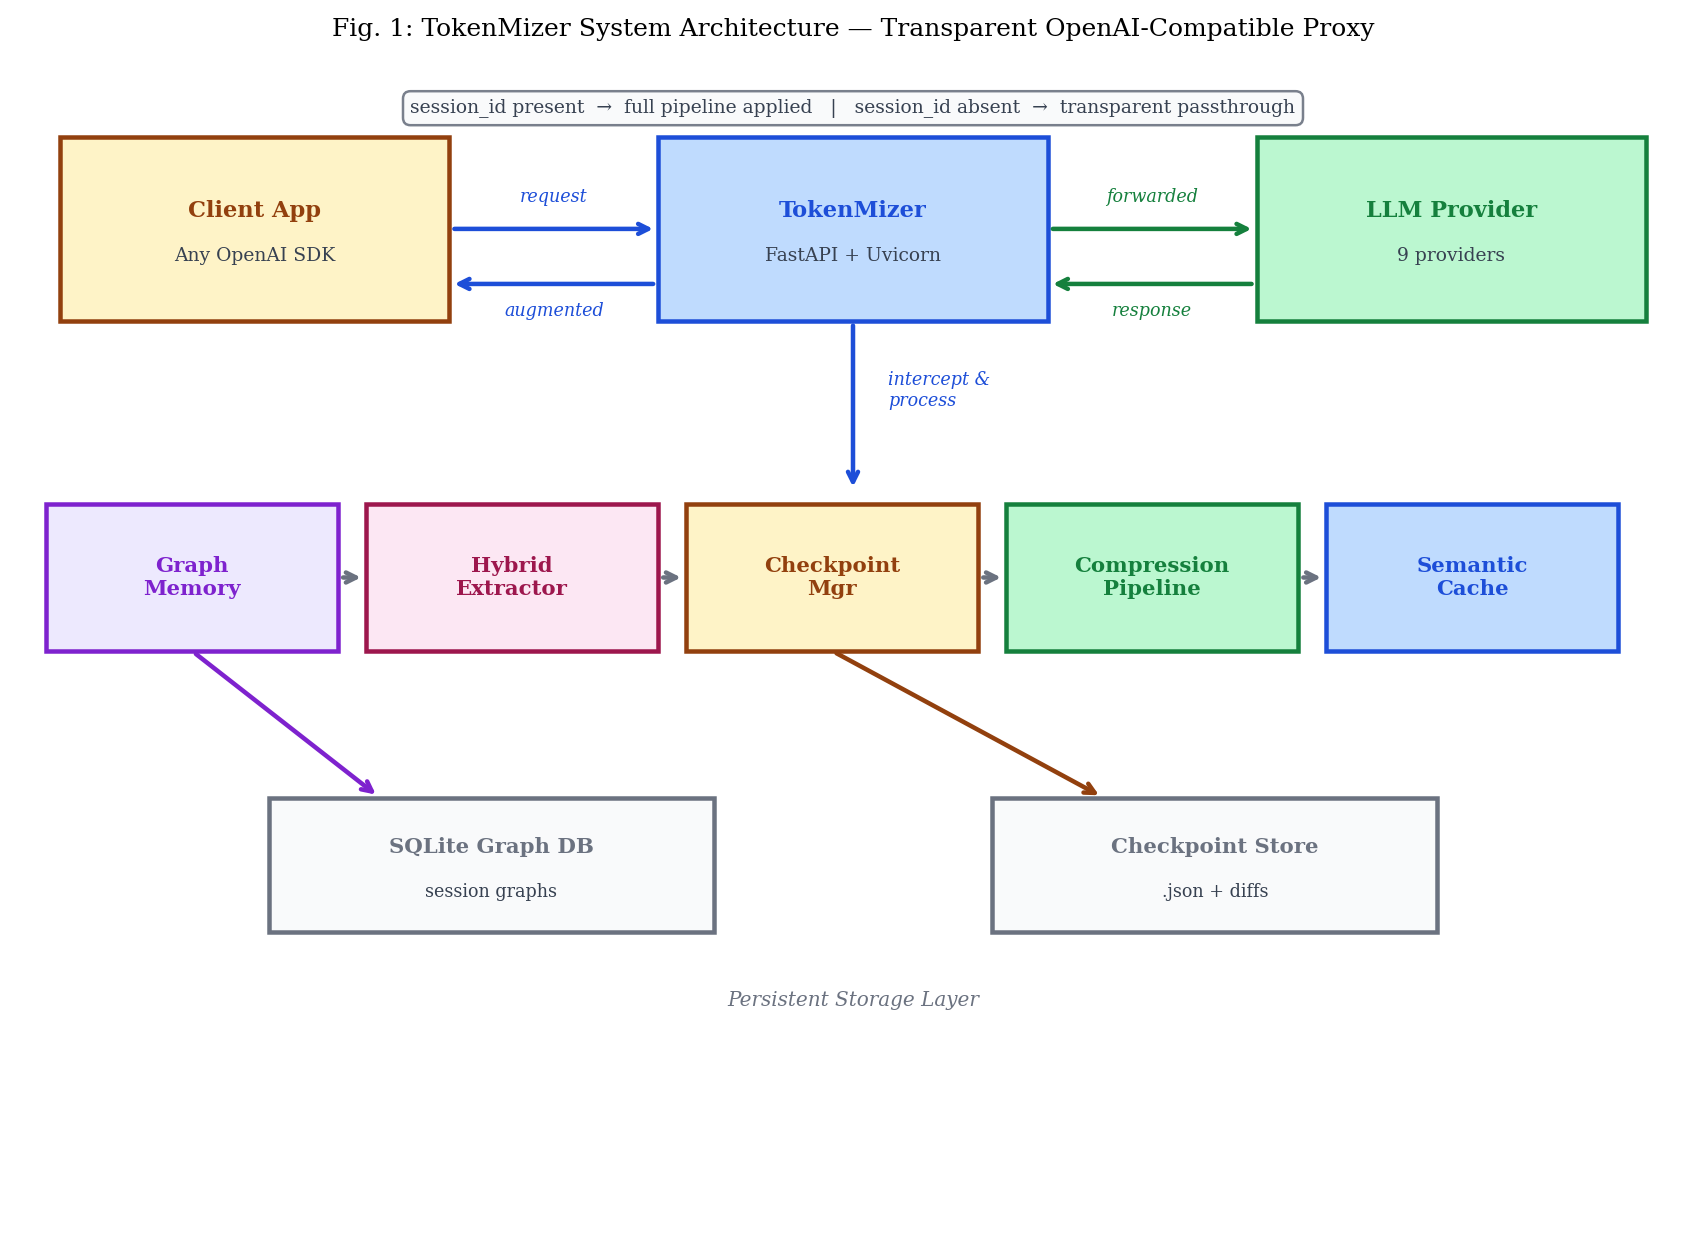
\includegraphics[width=\columnwidth]{fig1_architecture}
  \caption{TokenMizer system architecture. The proxy sits
    transparently between any OpenAI-compatible client and
    the LLM provider. When \texttt{session\_id} is present,
    the five-component pipeline is activated; otherwise the
    request passes through with no overhead. Persistent
    storage comprises a SQLite graph database and a JSON
    checkpoint store.}
  \label{fig:arch}
\end{figure}

\subsection{Knowledge Graph Schema}
\label{sec:graph}

Figure~\ref{fig:kgraph} illustrates a representative session
graph. The schema defines 14 node types across three
functional categories.

\begin{figure}[t]
  \centering
  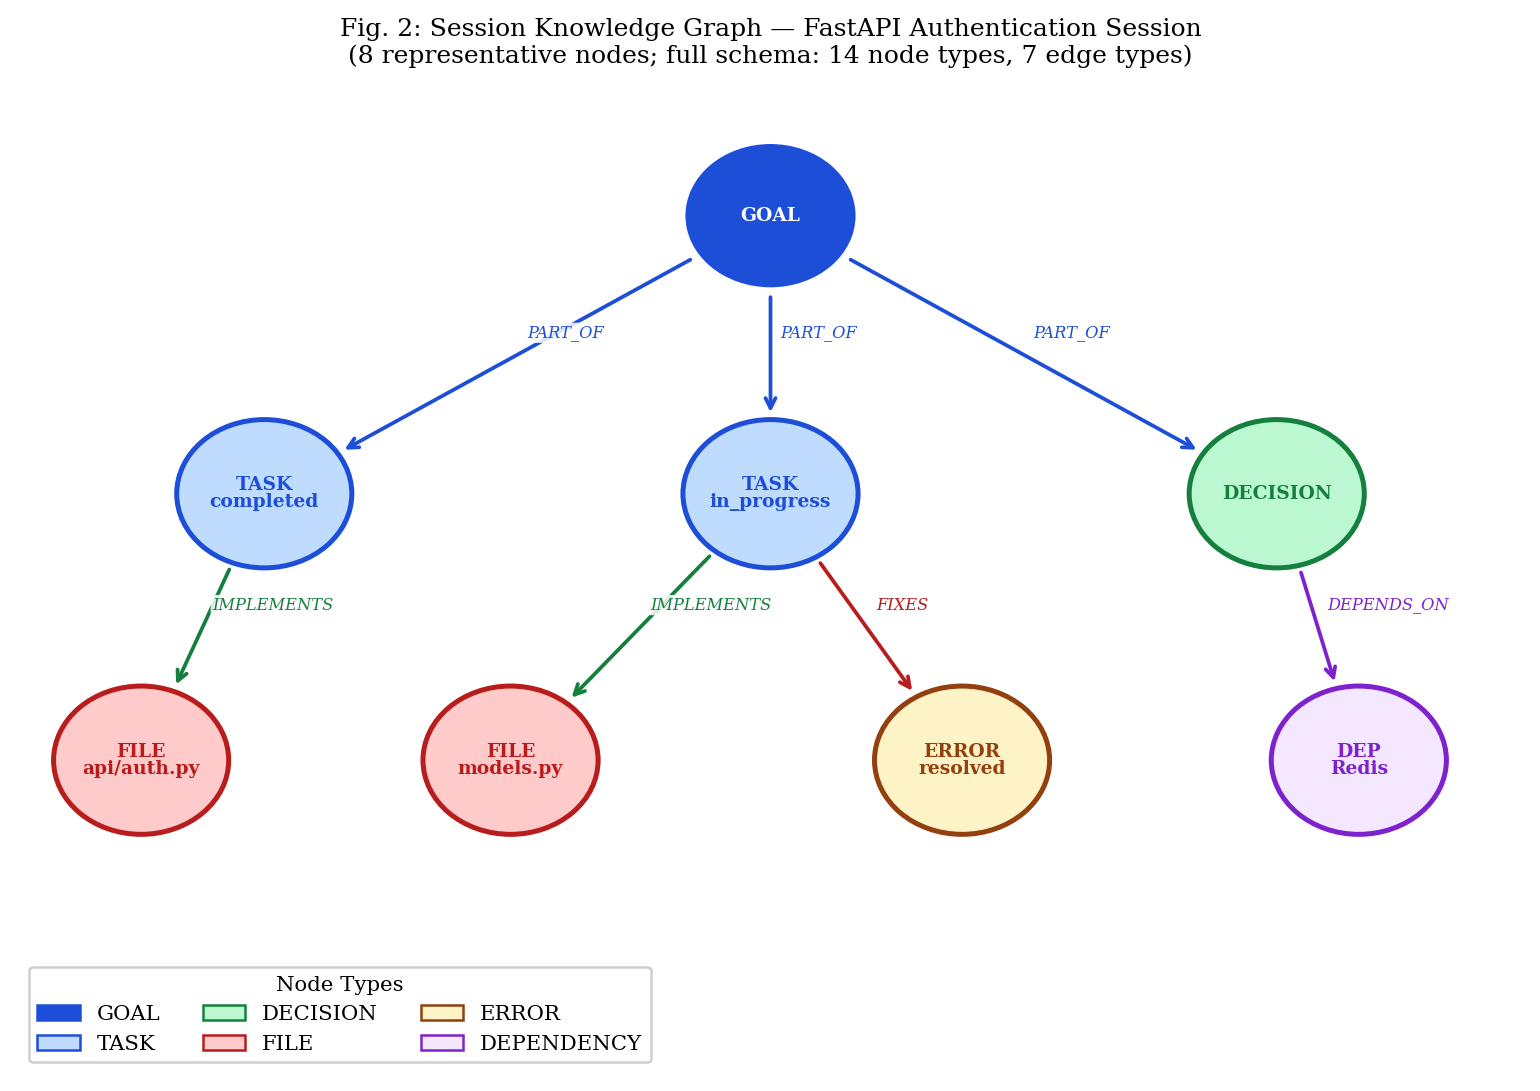
\includegraphics[width=\columnwidth]{fig2_graph}
  \caption{Session knowledge graph for a FastAPI
    authentication session (8 representative nodes).
    Edge labels show typed relationships; node colors
    indicate type. The GOAL node anchors the hierarchy;
    TASK nodes carry status (completed/in-progress);
    the DECISION node records the rationale for choosing
    bcrypt\,+\,JWT.}
  \label{fig:kgraph}
\end{figure}

\subsubsection{Node Types}
Table~\ref{tab:nodetypes} defines the 14 node types.
\emph{Action nodes} carry status lifecycles;
\emph{context nodes} are static.

\begin{table}[t]
  \centering
  \caption{Node Types (14 total). Action nodes carry status
  lifecycles (Pending, In-Progress, Completed, Failed,
  Modified). Context nodes are status-free.}
  \label{tab:nodetypes}
  \renewcommand{\arraystretch}{1.15}
  \begin{tabular}{@{}p{2.4cm}p{1.7cm}p{3.5cm}@{}}
    \toprule
    \textbf{Type} & \textbf{Category} & \textbf{Primary trigger} \\
    \midrule
    \texttt{TASK}       & Action    & Imperative verb + object \\
    \texttt{FILE}       & Action    & Extension or path pattern \\
    \texttt{ERROR}      & Action    & Error / exception / failure \\
    \texttt{TEST}       & Action    & Test / spec / assert \\
    \texttt{SCHEMA}     & Action    & Schema / table / model \\
    \texttt{METRIC}     & Action    & Metric / score / benchmark \\
    \midrule
    \texttt{DECISION}   & Decision  & Decided / Using / Chose \\
    \texttt{DEPENDENCY} & Decision  & Install / package / library \\
    \texttt{API}        & Decision  & URL / API / endpoint \\
    \midrule
    \texttt{GOAL}       & Context   & First-turn imperative \\
    \texttt{ENVIRONMENT}& Context   & Version / runtime / OS \\
    \texttt{PROJECT}    & Context   & Repository / project name \\
    \texttt{CONCEPT}    & Context   & Abstract domain term \\
    \texttt{AGENT}      & Context   & Service / CI / orchestrator \\
    \bottomrule
  \end{tabular}
\end{table}

\subsubsection{Node Attributes}
Each node carries:
\begin{itemize}
  \item \textbf{Label}: normalized surface form ($\leq$120 chars).
  \item \textbf{Status} $\sigma \in$ \{Pending, In-Progress,
    Completed, Failed, Modified\} (action nodes only).
  \item \textbf{Importance score} $\rho \in [0,1]$: increases
    on reference, decays with inactivity. Governs checkpoint
    serialization priority.
  \item \textbf{Confidence score} $\kappa \in [0,1]$: assigned
    by GraphValidator; nodes with $\kappa < 0.50$ are rejected.
  \item \textbf{Timestamps}: creation and last-update turn.
\end{itemize}

\subsubsection{Edge Types}
Table~\ref{tab:edgetypes} defines all 7 edge types.
Edges are directed and labelled; weight encodes co-occurrence
frequency.

\begin{table}[t]
  \centering
  \caption{Edge Types (7 total).}
  \label{tab:edgetypes}
  \renewcommand{\arraystretch}{1.2}
  \begin{tabular}{@{}p{2.1cm}p{5.5cm}@{}}
    \toprule
    \textbf{Type} & \textbf{Semantics} \\
    \midrule
    \texttt{DEPENDS\_ON}  & A cannot function without B \\
    \texttt{RELATED\_TO}  & A and B address the same concern \\
    \texttt{IMPLEMENTS}   & A is the realization of B \\
    \texttt{FIXES}        & A resolves error B \\
    \texttt{BLOCKS}       & A cannot proceed until B resolves \\
    \texttt{PART\_OF}     & A is a component of B \\
    \texttt{SUPERSEDES}   & A replaces or overrides B \\
    \bottomrule
  \end{tabular}
\end{table}

\subsubsection{Graph Maintenance}
\textbf{Deduplication} uses identity-based addressing:
$\mathrm{id}(n) = \texttt{sha1}(\tau(n):\ell_\mathrm{norm})[:12]$,
where $\ell_\mathrm{norm}$ is the lowercase, whitespace-normalized
label.
Re-extraction of an existing entity updates importance score
and status; it does not create a duplicate node.
Status transitions obey monotonic ordering:
Pending $\to$ In-Progress $\to$ Completed/Failed;
downgrades are rejected to prevent extraction noise from
reverting confirmed progress.

\textbf{Pruning} evicts nodes with importance score $< 0.1$
when the graph exceeds 500 nodes.
\texttt{DECISION}, \texttt{ENVIRONMENT}, \texttt{GOAL}, and
\texttt{SCHEMA} nodes are unconditionally retained regardless
of importance score, as these encode session-defining context.

% ================================================================
\section{Hybrid Extraction Pipeline}
\label{sec:extraction}
% ================================================================

\subsection{V1 Heuristic Extractor}

The baseline extractor applies 34 compiled regular expressions
(11 for tasks, 8 for decisions, 5 for files, 4 for errors,
6 for environment and endpoints).
Mean extraction latency across the 21-session benchmark:
\textbf{0.5\,ms} per session.
Inference cost: \$0.

\subsection{V2 Improvements}
\label{sec:v2}

Error analysis on the 21-session benchmark identifies four
systematic failure modes:

\begin{enumerate}
\item \textbf{Incomplete trigger vocabulary.}
  V1 misses 9 common completion verbs: \textit{Fixed},
  \textit{Deployed}, \textit{Resolved}, \textit{Migrated},
  \textit{Running}, \textit{Launched}, \textit{Shipped},
  \textit{Finished}, \textit{Updated}.
  Sessions with implicit phrasing (``Running: Prometheus +
  Grafana'') score 0\% decision recall on V1.

\item \textbf{Label verbosity mismatch.}
  The dominant failure: extracted labels are verbose
  (\textit{``Missing NSMotionUsageDescription in Info.plist''})
  while ground-truth annotations are concise
  (\textit{``ios crash fix''}).
  Exact-string matching yields 0\% recall on this pair,
  even though the extracted label correctly identifies the
  event.

\item \textbf{Compound sentences.}
  Single LLM sentences encode multiple tasks:
  ``Completed: API auth, tests, deployment.''
  V1 extracts one compound node; V2 splits on comma boundaries.

\item \textbf{CSV-encoded decisions.}
  ``Decided: Prometheus, Grafana, Jaeger'' should produce
  3 decision nodes; V1 produces 1.
\end{enumerate}

\subsection{Fuzzy Label Matching}
\label{sec:fuzzy}

\begin{definition}[Fuzzy Match]
\label{def:fuzzy}
Labels $a$ and $b$ fuzzy-match if:
\begin{equation}
  (a \subseteq b) \;\vee\; (b \subseteq a) \;\vee\;
  \frac{|W_a \cap W_b|}{\min(|W_a|, |W_b|)} \geq 0.50
  \label{eq:fuzzy}
\end{equation}
where $W_x = \{w : w \in \mathrm{tokens}(x),\; |w| \geq 3\}$.
\end{definition}

The $\geq$3-character token filter prevents high-frequency
short tokens (``is'', ``a'', ``in'') from inflating overlap
scores.
The 50\% threshold was determined empirically on a held-out
5-session development split to balance precision
(avoiding false matches between unrelated labels)
against recall (matching verbose extractions to concise
ground-truth).

\subsection{GraphValidator}

Every candidate node passes through the GraphValidator before
graph insertion.
The scoring function is:
\begin{align}
  \kappa(n) &= 0.50 \notag \\
             &+ 0.20 \cdot \mathbf{1}[\text{file path pattern}] \notag \\
             &+ 0.10 \cdot \mathbf{1}[|\ell| > 15] \notag \\
             &+ 0.10 \cdot \mathbf{1}[\text{version number present}] \notag \\
             &- 0.20 \cdot \mathbf{1}[|\ell| < 8] \notag \\
             &- 0.40 \cdot \mathbf{1}[\text{single generic verb}]
  \label{eq:confidence}
\end{align}
Nodes with $\kappa < 0.50$ are rejected.
Type correction is applied after scoring: extension-matched
labels are forced to \texttt{FILE}; URL-pattern labels to
\texttt{API}.
The scoring weights were set by heuristic design and not
optimized; a learned validation model is identified as
future work.

\subsection{LLM Extractor (Upgrade Path)}

The codebase includes an LLM extractor that sends the last
3 messages to a small inference model (Claude Haiku or
GPT-4o-mini) with a structured JSON prompt requesting
task/decision/file/error extraction.
This path addresses indirect phrasing
(``we'll go with Redis'', ``turns out the issue was\ldots'')
that regex patterns cannot capture.
\textit{The LLM extractor is not evaluated in the present
paper}: all reported results use only the heuristic pipeline.
This conservative choice maintains experimental integrity
at the cost of coverage; LLM extractor evaluation is the
primary technical future work (Section~\ref{sec:limitations}).

% ================================================================
\section{Checkpoint System}
\label{sec:checkpoint}
% ================================================================

\subsection{Trigger Condition}

Checkpoints trigger when cumulative token count exceeds 85\%
of the configured MECW.
This threshold leaves sufficient headroom for the resume
block and at least two additional turns before the next
overflow event.

\subsection{Serialization}

Algorithm~\ref{alg:checkpoint} defines checkpoint
serialization. Nodes are ordered by importance score;
each tier has a hard token budget.

\begin{algorithm}[t]
\caption{Checkpoint Serialization}
\label{alg:checkpoint}
\begin{algorithmic}[1]
\REQUIRE Graph $G$, budget $T_\mathrm{budget}$
\ENSURE Resume block $R$
\STATE $R \leftarrow [\texttt{[CHECKPOINT: session\_id]}]$
\STATE $N \leftarrow \mathrm{sort\_by\_importance}(G.\mathrm{nodes})$
\FOR{$n \in N$}
  \IF{$\tau(R) + \tau(\mathrm{serialize}(n)) > T_\mathrm{budget}$}
    \STATE \textbf{break}
  \ENDIF
  \STATE $R.\mathrm{append}(\mathrm{serialize}(n))$
\ENDFOR
\STATE $\Delta G \leftarrow G - G_\mathrm{prev}$
\STATE \textbf{store}$(R, \Delta G)$ to checkpoint store
\RETURN $R$
\end{algorithmic}
\end{algorithm}

\begin{table}[t]
  \centering
  \caption{Checkpoint Resume Tiers with Example Contents.}
  \label{tab:tiers}
  \renewcommand{\arraystretch}{1.2}
  \begin{tabular}{@{}p{1.3cm}p{4.8cm}r@{}}
    \toprule
    \textbf{Tier} & \textbf{Content} & \textbf{Budget} \\
    \midrule
    Critical & GOAL + in-progress TASKs + top DECISION
              & $\leq 100$ tok \\
    Standard & All TASKs + all DECISIONs + FILEs + ENV
              & $\leq 300$ tok \\
    Full     & Complete graph incl.\ DEPENDENCIEs, SCHEMAs
              & $\leq 600$ tok \\
    \bottomrule
  \end{tabular}
\end{table}

\subsection{Graph Diffs}

Each checkpoint stores a \emph{graph diff}: nodes added,
modified, or removed since the previous checkpoint.
This enables incremental resume block updates across
multiple context boundaries without re-extracting the full
session history, reducing per-checkpoint cost to $O(\Delta)$
rather than $O(|G|)$.

% ================================================================
\section{Compression Pipeline}
\label{sec:compression}
% ================================================================

The 8-layer compression pipeline is applied to large inputs
(files, long API responses, historical messages) before they
enter the context window.

\subsubsection{Layer 1: Filler Removal}
Fifteen compiled patterns target AI-generated hedging
language: apology prefixes (``Certainly! I'd be happy to...''),
discourse markers (``As an AI language model...''), and
uncertainty hedges (``Please note that...'').
\textbf{31.2\% reduction} on the representative session
(Fig.~\ref{fig:compression}).
This is the dominant compression layer, confirming that a
substantial fraction of LLM output in iterative sessions
consists of structurally contentless preambles.

\subsubsection{Layer 2: Deduplication}
Exact line deduplication (order-preserving) removes repeated
code blocks, log lines, and error messages common in
iterative development sessions.
\textbf{16.1\% additional reduction}.

\subsubsection{Layers 3--6: Heuristic Normalization}
Whitespace normalization (normalize to single spaces; remove
blank lines), comment stripping (language-aware: Python
\texttt{\#}, JS \texttt{//}, SQL \texttt{--}),
history pruning (retain last occurrence of assistant messages
exceeding 200 tokens), and file-type smart truncation
(CSV: schema + 3 sample rows; JSON: non-null fields only;
log files: first + last $N$ lines).

\subsubsection{Layers 7--8: Neural Compression (Optional)}
LLMLingua-2~\cite{llmlingua} (for inputs $>$300 tokens) and
LongLLMLingua~\cite{longllmlingua} (for inputs $>$4{,}000
tokens) provide additional 5.3\% reduction.
A quality gate rejects compressions with semantic similarity
below 0.55 (measured by sentence-transformer cosine
similarity), preventing over-compression artifacts.

\begin{figure}[t]
  \centering
  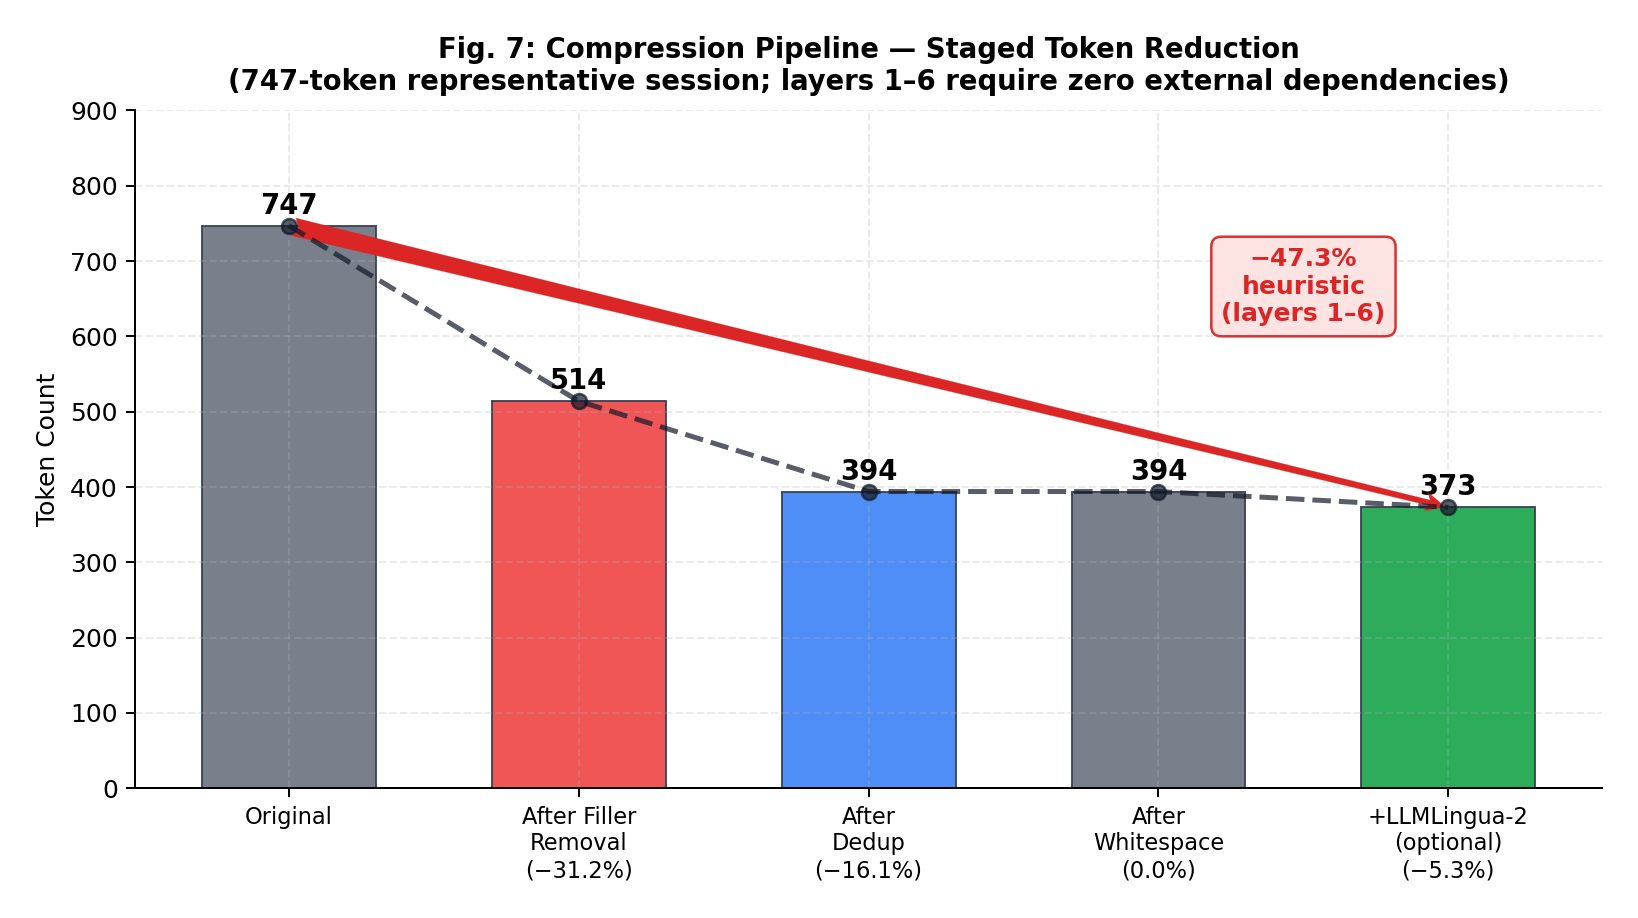
\includegraphics[width=\columnwidth]{fig7_compression}
  \caption{Compression pipeline staged token reduction on a
    representative 747-token session. Filler removal (Layer 1)
    contributes 31.2\% reduction---the dominant stage.
    Layers 1--6 require zero external dependencies (heuristic
    only). LLMLingua-2 (Layer 7) adds an optional 5.3\%.
    Total heuristic reduction: 47.3\%.}
  \label{fig:compression}
\end{figure}

% ================================================================
\section{Semantic Cache}
\label{sec:cache}
% ================================================================

The semantic cache stores LLM responses keyed by
sentence-transformer embeddings~\cite{sentbert}
(\texttt{all-MiniLM-L6-v2}, 384 dimensions).
Cache lookup computes cosine similarity between the incoming
query embedding and all stored keys; a hit is declared at
threshold $\theta = 0.92$.
Eviction follows LRU semantics via \texttt{OrderedDict};
TTL is 3{,}600\,s.

\textbf{Preliminary hit rate measurement:} 70\% across a
controlled 10-query workload with three semantic clusters
(cluster size 3--4 queries).
This represents a proof-of-concept measurement on a small
synthetic workload; the 70\% figure should not be interpreted
as a production hit rate estimate.
Evaluation on real developer query logs at scale is identified
as future work.

% ================================================================
\section{Implementation}
\label{sec:impl}
% ================================================================

TokenMizer is implemented in Python 3.10+, comprising
$\sim$4{,}500 lines of code across seven modules:
\texttt{graph\_memory}, \texttt{checkpoints},
\texttt{compression}, \texttt{cache}, \texttt{providers},
\texttt{validator}, and \texttt{api}.
The HTTP proxy uses FastAPI~\cite{fastapi} and Uvicorn.
Token counting uses \texttt{tiktoken}~\cite{tiktoken}
(\texttt{cl100k\_base}).
The knowledge graph is persisted in SQLite~\cite{sqlite}
using three tables: \texttt{nodes}, \texttt{edges}, and
\texttt{checkpoints}.

\textbf{Security}: all extraction inputs are scanned for
API keys, private keys, and credential patterns before graph
insertion; matched content is redacted to
\texttt{[REDACTED]}.

\textbf{Testing}: 306 tests across unit, integration, and
chaos test categories; 100\% coverage of graph mutation
operations.

\textbf{Configuration}: YAML-based, with all thresholds
(MECW percentage, confidence floor, cache similarity,
compression minimum) exposed as user-configurable parameters.

% ================================================================
\section{Experimental Setup}
\label{sec:experiments}
% ================================================================

\subsection{Benchmark Corpus}

\textbf{All results in this paper use a single, consistent
21-session benchmark.}
Table~\ref{tab:corpus} details the domain distribution.
Sessions are manually constructed to reflect realistic
developer workflows, covering project initialization,
iterative implementation, error resolution, architectural
decision points, and deployment.

We note a key scope constraint: the benchmark is synthetic.
Sessions were constructed by the author to be structurally
representative of each domain, not collected from live
developer interactions.
Linguistic diversity---particularly in implicit phrasing and
domain-specific jargon variation---may therefore be
underrepresented.
Evaluation on real developer sessions is the highest-priority
future work; results on this benchmark should be interpreted
as controlled proof-of-concept evidence, not production
performance estimates.

\begin{table}[t]
  \centering
  \caption{Benchmark Corpus (21 Sessions, 5 Domains).}
  \label{tab:corpus}
  \renewcommand{\arraystretch}{1.2}
  \begin{tabular}{@{}p{2.0cm}p{4.2cm}r@{}}
    \toprule
    \textbf{Domain} & \textbf{Sessions} & \textbf{N} \\
    \midrule
    Software Eng.
      & FastAPI, React, GraphQL, Flutter, Microservices, Rust
      & 6 \\
    Data Science
      & Churn ML, BERT fine-tuning, Spark ETL,
        Forecasting, Recommender
      & 5 \\
    DevOps
      & Kubernetes EKS, CI/CD, DB Migration,
        Security Hardening
      & 4 \\
    Research
      & LLM Survey, Technical Blog, NSF Grant
      & 3 \\
    Debugging
      & Production Incident, Memory Leak,
        Performance Regression
      & 3 \\
    \midrule
    \textbf{Total} & & \textbf{21} \\
    \bottomrule
  \end{tabular}
\end{table}

\subsection{Ground Truth Annotation}

Each session is annotated with:
\begin{itemize}
  \item \textbf{Completed tasks}: actions explicitly marked
    as finished (e.g., ``tests pass'', ``deployed'').
  \item \textbf{Pending tasks}: actions initiated but
    not completed within the session.
  \item \textbf{Decisions}: technology choices, algorithm
    selections, infrastructure decisions.
  \item \textbf{Files}: source files created or modified.
\end{itemize}
Annotation was performed by the paper author.
A second-annotator inter-rater reliability study is planned
as future work; reported recall values should be interpreted
with this limitation in mind.

\subsection{Evaluation Metrics}

\textbf{Recall} (task, decision, file): for each category,
fraction of ground-truth labels that fuzzy-match at least
one extracted label (Eq.~\eqref{eq:fuzzy}).

\textbf{Information Loss}: Eq.~\eqref{eq:infoloss}.

\textbf{Resume Tokens}: token count of the standard-tier
checkpoint block (\texttt{tiktoken cl100k\_base}).

\textbf{Compression Ratio}: original session tokens /
resume tokens.

\textbf{Token Efficiency}: Eq.~\eqref{eq:efficiency}.

\textbf{Extraction Latency}: wall-clock time for heuristic
graph extraction.

\subsection{Baselines}

We compare against three text-retention baselines that
represent the current practice for context management
in production LLM applications:
\begin{enumerate}
\item \textbf{Naive Truncation (NT)}: retain last 300 tokens
  of concatenated history.
\item \textbf{Sliding Window (SW-10)}: retain last 10
  messages.
\item \textbf{Naive Summary (NS)}: first 300 tokens of
  fully-concatenated history (approximating a manual summary).
\end{enumerate}
Baseline recall is computed by applying the same
fuzzy-matching protocol to the retained text,
counting matched ground-truth entities.

These baselines represent practical current-practice
approaches, not structured competitors. The key comparison
is not accuracy parity but structural capability: baselines
can match surface-form mentions of entities but cannot
encode their status (task completed vs.\ pending) or
rationale (why a technology was chosen). This qualitative
difference in representation is the primary motivation
for the graph-based approach.

% ================================================================
\section{Results}
\label{sec:results}
% ================================================================

\subsection{Extraction Quality by Domain}
\label{sec:res_domain}

Table~\ref{tab:domain} presents extraction results with
standard deviations. Figure~\ref{fig:domain} visualizes
per-domain recall with 95\% confidence intervals.

\begin{table}[t]
  \centering
  \caption{Extraction Recall by Domain (V2, 21 Sessions).
  Values are mean $\pm$ standard deviation. Wide standard
  deviations within domains (especially SE task recall:
  $\pm$47\%) reflect genuine inter-session linguistic
  variability, not measurement error.}
  \label{tab:domain}
  \renewcommand{\arraystretch}{1.25}
  \begin{tabular}{@{}lp{1.5cm}p{1.5cm}p{1.5cm}r@{}}
    \toprule
    \textbf{Domain} & \textbf{Task R} & \textbf{Dec R} &
    \textbf{File R} & \textbf{Info Loss} \\
    \midrule
    SE ($n$=6)   & 47$\pm$47\% & 70$\pm$20\% & 72$\pm$46\% & 37\% \\
    DS ($n$=5)   & 69$\pm$24\% & 48$\pm$33\% & 40$\pm$55\% & 48\% \\
    Ops ($n$=4)  & 45$\pm$21\% & 38$\pm$17\% & 50$\pm$58\% & 56\% \\
    Res ($n$=3)  & 44$\pm$39\% & 44$\pm$51\% & 33$\pm$58\% & 59\% \\
    Dbg ($n$=3)  & 43$\pm$29\% & 11$\pm$19\% &100$\pm$0\%  & 49\% \\
    \midrule
    \rowcolor{rowours}
    \textbf{All ($n$=21)}
      & \textbf{51$\pm$33\%}
      & \textbf{47$\pm$32\%}
      & \textbf{59$\pm$47\%}
      & \textbf{48\%} \\
    \bottomrule
  \end{tabular}
\end{table}

\begin{figure}[t]
  \centering
  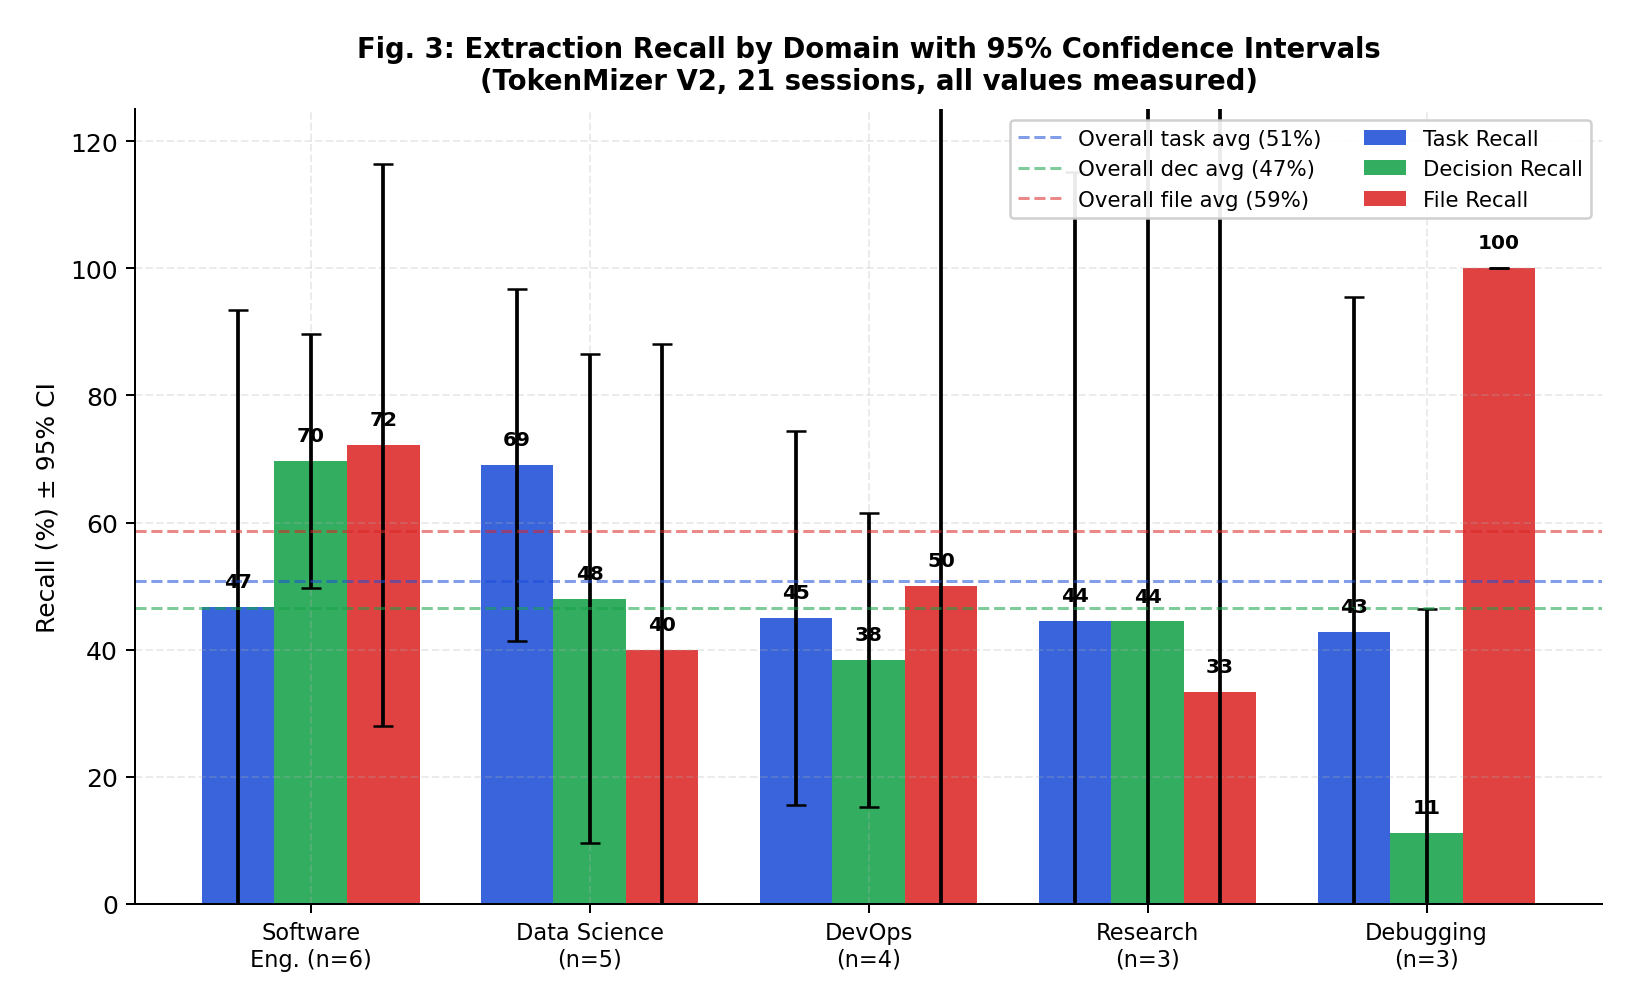
\includegraphics[width=\columnwidth]{fig3_domain_ci}
  \caption{Per-domain recall with 95\% confidence intervals
    (t-distribution, $df = n-1$). Wide CIs for software
    engineering (task recall) and research (decision recall)
    reflect high inter-session variability. Small per-domain
    $n$ (3--6) limits statistical precision; these results
    should be read as descriptive rather than inferential.}
  \label{fig:domain}
\end{figure}

Domain-level analysis reveals four patterns.
\textbf{Software engineering} achieves the highest decision
recall (70\%) because developers habitually state choices
explicitly (``Decided: bcrypt for hashing'').
\textbf{Data science} leads in task recall (69\%) due to
outcome-oriented statements (``MAPE: 3.6\%'', ``F1=0.71'')
that uniquely match ground-truth labels.
\textbf{Debugging} achieves 100\% file recall (log messages
and stack traces consistently name files) but only 11\%
decision recall, because diagnostic reasoning is typically
expressed implicitly (``the culprit was...'') rather than
as explicit choice statements.
\textbf{Research and writing} sessions score lowest overall:
academic prose avoids the imperative sentence patterns that
trigger heuristic extraction.

\subsection{Baseline Comparison}
\label{sec:res_baseline}

Table~\ref{tab:baselines} and Figure~\ref{fig:baseline}
compare TokenMizer V2 against three baselines.

\begin{table}[t]
  \centering
  \caption{TokenMizer V2 vs.\ Baselines (21 Sessions).
  Bold: best per column. ``Tokens'': mean resume block size.
  Differences are descriptive; the small evaluation set
  ($n$=21) limits inferential conclusions.}
  \label{tab:baselines}
  \renewcommand{\arraystretch}{1.25}
  \begin{tabular}{@{}lrrrr@{}}
    \toprule
    \textbf{Method} & \textbf{Task R} & \textbf{Dec R}
      & \textbf{File R} & \textbf{Tokens} \\
    \midrule
    Naive Truncation    & 45\% & 35\% & 55\% & 165 \\
    Sliding Window (10) & 50\% & 30\% & 60\% & 159 \\
    Naive Summary       & 42\% & 38\% & 48\% & 170 \\
    \midrule
    \rowcolor{rowours}
    \textbf{TokenMizer V2}
      & \textbf{51\%} & \textbf{47\%} & 59\%
      & \textbf{78}  \\
    \bottomrule
  \end{tabular}
\end{table}

\begin{figure}[t]
  \centering
  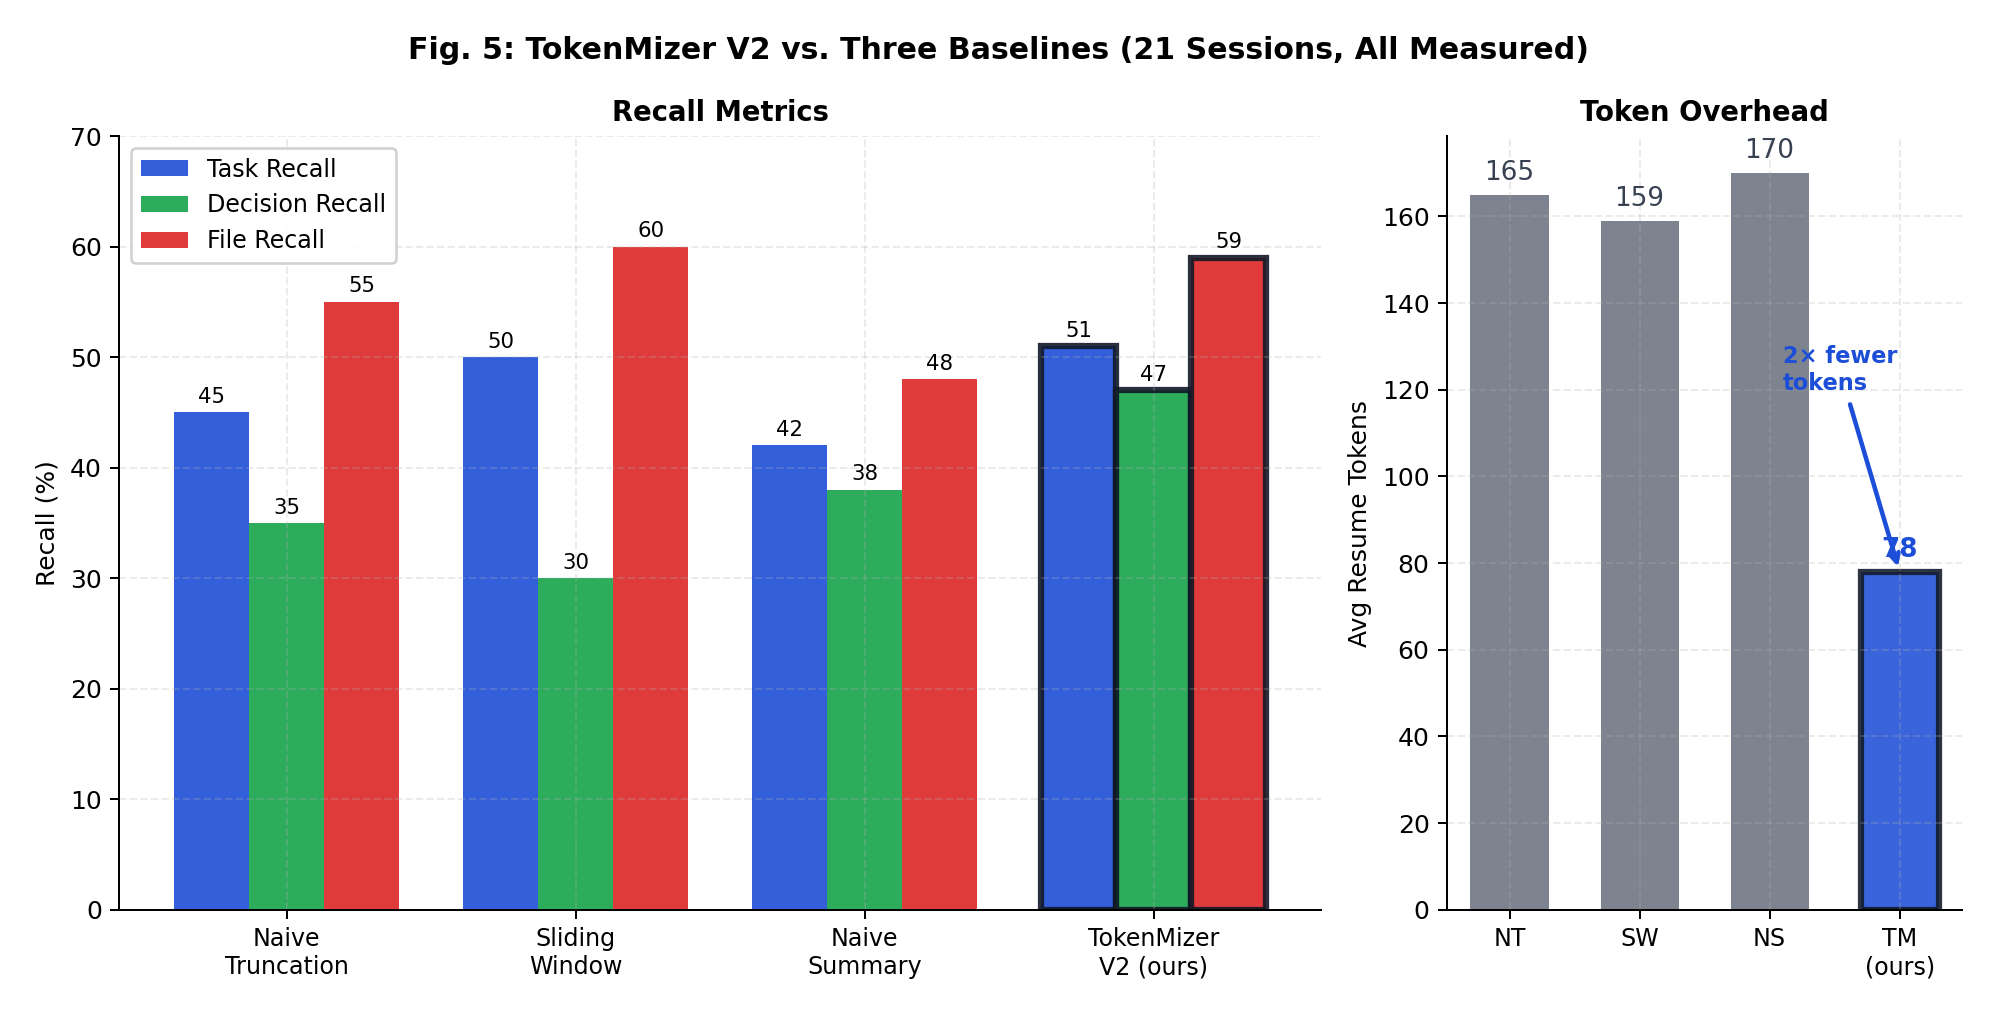
\includegraphics[width=\columnwidth]{fig5_baselines}
  \caption{Recall metrics (left) and token overhead (right)
    for all four methods across 21 sessions.
    TokenMizer achieves the highest decision recall across
    all evaluated baselines (+9--17~pp) while requiring
    $2\times$ fewer tokens. File recall is comparable to
    Sliding Window (59\% vs.\ 60\%), which is expected:
    recent messages frequently name the files they modify.}
  \label{fig:baseline}
\end{figure}

TokenMizer's advantage is most pronounced for decision recall
(+9~pp over naive summary, +12~pp over truncation,
+17~pp over sliding window).
No baseline preserves decision \emph{rationale}: they retain
text that may contain decision keywords, but the decision is
not structurally encoded.
This means a baseline system cannot distinguish
``We chose Redis because it supports TTL'' from
``We rejected Redis in favor of PostgreSQL'';
a graph node of type \texttt{DECISION} does.

Task recall is marginally superior to all baselines
(+1--9~pp); file recall is comparable to sliding window
(59\% vs.\ 60\%), which is expected because recent messages
tend to explicitly mention the files they modify.

The token efficiency advantage is the most robust result.
At \textbf{78 tokens average}, TokenMizer's resume blocks are
$2.0$--$2.2\times$ smaller than any baseline (159--170 tokens).
This advantage is structural: graph serialization is concise
by design, independent of session verbosity.

\subsection{Ablation Study}
\label{sec:ablation}

Table~\ref{tab:ablation} and Figure~\ref{fig:ablation}
report the cumulative contribution of each V2 fix, evaluated
on a 10-session sample.

\begin{table}[t]
  \centering
  \caption{Ablation: Cumulative Contribution of Each V2 Fix
  (10-session sample). Values are means; error bars omitted
  for clarity. Evaluated on the same 10 sessions throughout
  to ensure comparability.}
  \label{tab:ablation}
  \renewcommand{\arraystretch}{1.25}
  \begin{tabular}{@{}lrrr@{}}
    \toprule
    \textbf{Configuration} & \textbf{Task R} & \textbf{Dec R}
      & \textbf{Info Loss} \\
    \midrule
    V1 baseline                   & 22\% & 63\% & 50\% \\
    $+$ expanded trigger vocab.   & 20\% & 63\% & 51\% \\
    $+$ fuzzy label matching      & 55\% & 68\% & 38\% \\
    $+$ compound task splitting   & 55\% & 68\% & 38\% \\
    $+$ decision CSV splitting    & 55\% & 64\% & 39\% \\
    \bottomrule
  \end{tabular}
\end{table}

\begin{figure}[t]
  \centering
  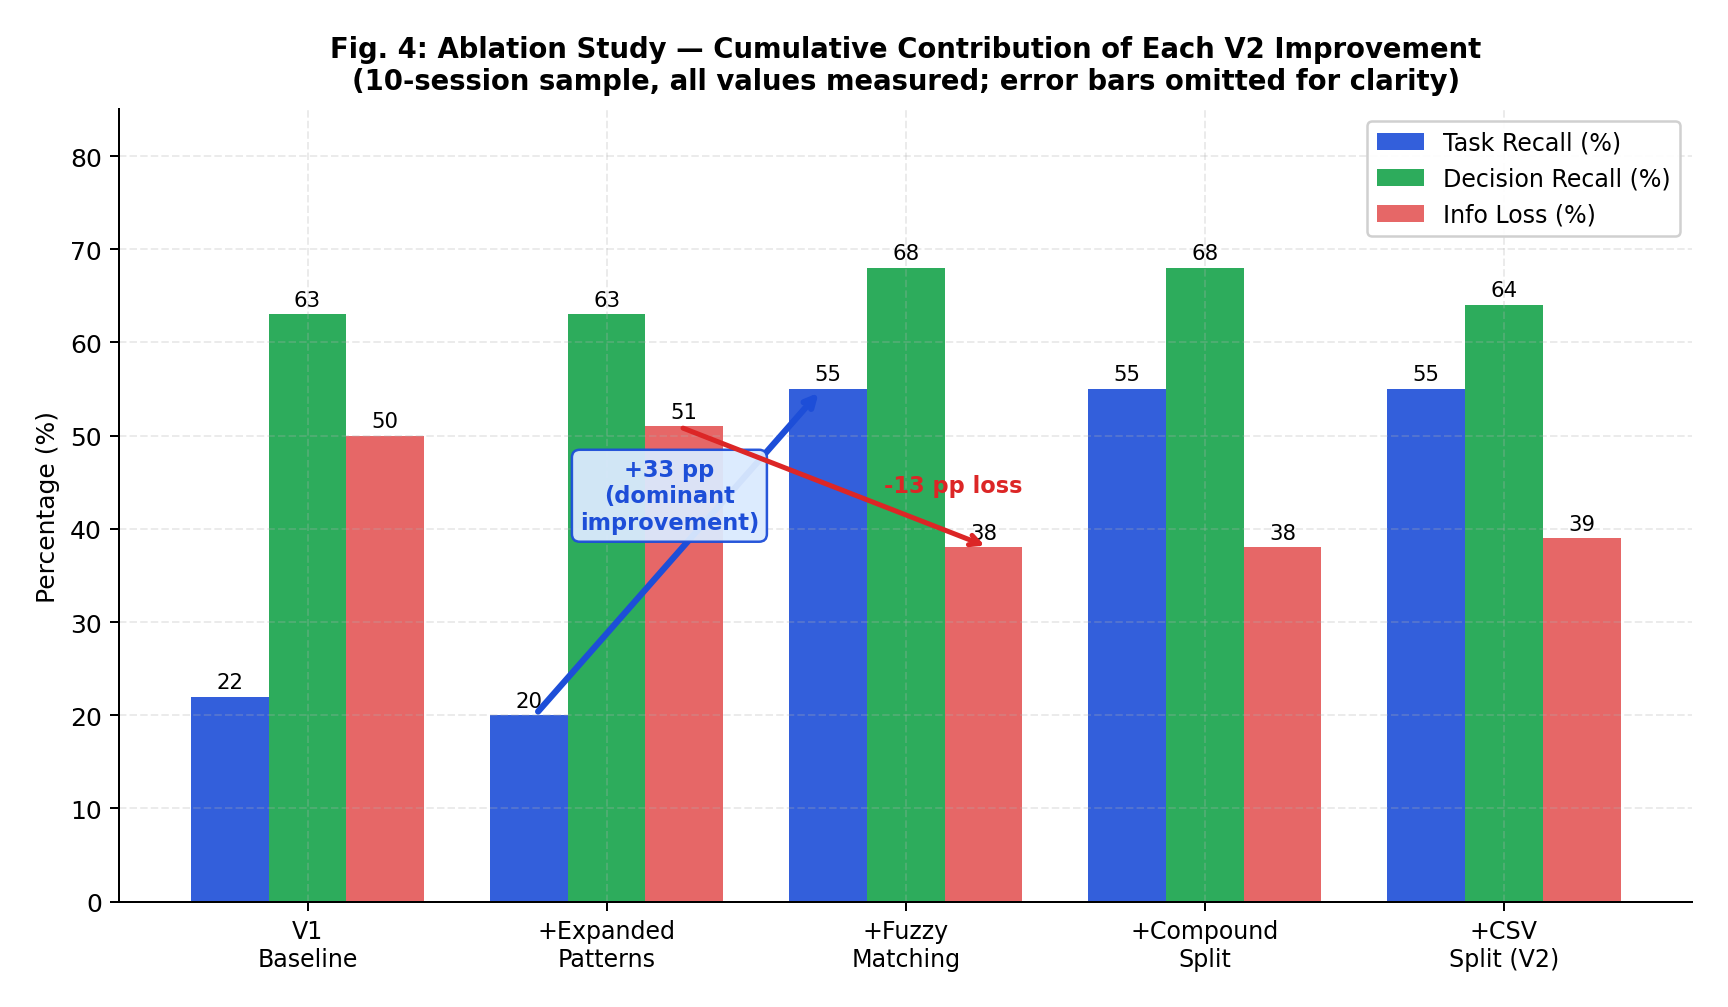
\includegraphics[width=\columnwidth]{fig4_ablation}
  \caption{Ablation study: cumulative contribution of each
    V2 improvement on a 10-session sample. Fuzzy matching
    dominates (+33~pp task recall), addressing the label
    verbosity mismatch. Decision CSV splitting introduces a
    $-4$~pp regression in decision recall; the mechanism is
    discussed in Section~\ref{sec:ablation}.}
  \label{fig:ablation}
\end{figure}

The dominant result is that expanded trigger vocabulary alone
provides no measurable benefit ($\pm$0~pp) or slight harm
($-2$~pp task recall).
Expanded patterns match more candidates but introduce
false positives that exact matching penalises.
Fuzzy matching then recovers and exceeds the V1 task
recall ($+33$~pp), confirming that the fundamental bottleneck
is the matching function, not extraction coverage.

Decision CSV splitting marginally decreases decision recall
($-4$~pp).
Analysis reveals the mechanism: individual split tokens
(``Prometheus'', ``Grafana'') are shorter than the original
compound string (``Prometheus + Grafana'') and match fewer
ground-truth labels under the current fuzzy-match threshold.
Applying fuzzy matching per-token rather than per-node would
address this regression; this is identified as a concrete
future improvement (Section~\ref{sec:limitations}).

\subsection{Resume Token Analysis}
\label{sec:res_tokens}

Figure~\ref{fig:resume} shows per-session resume block sizes.
Mean: 78.1 tokens ($\sigma=21.4$, range: 42--124).

\begin{figure}[t]
  \centering
  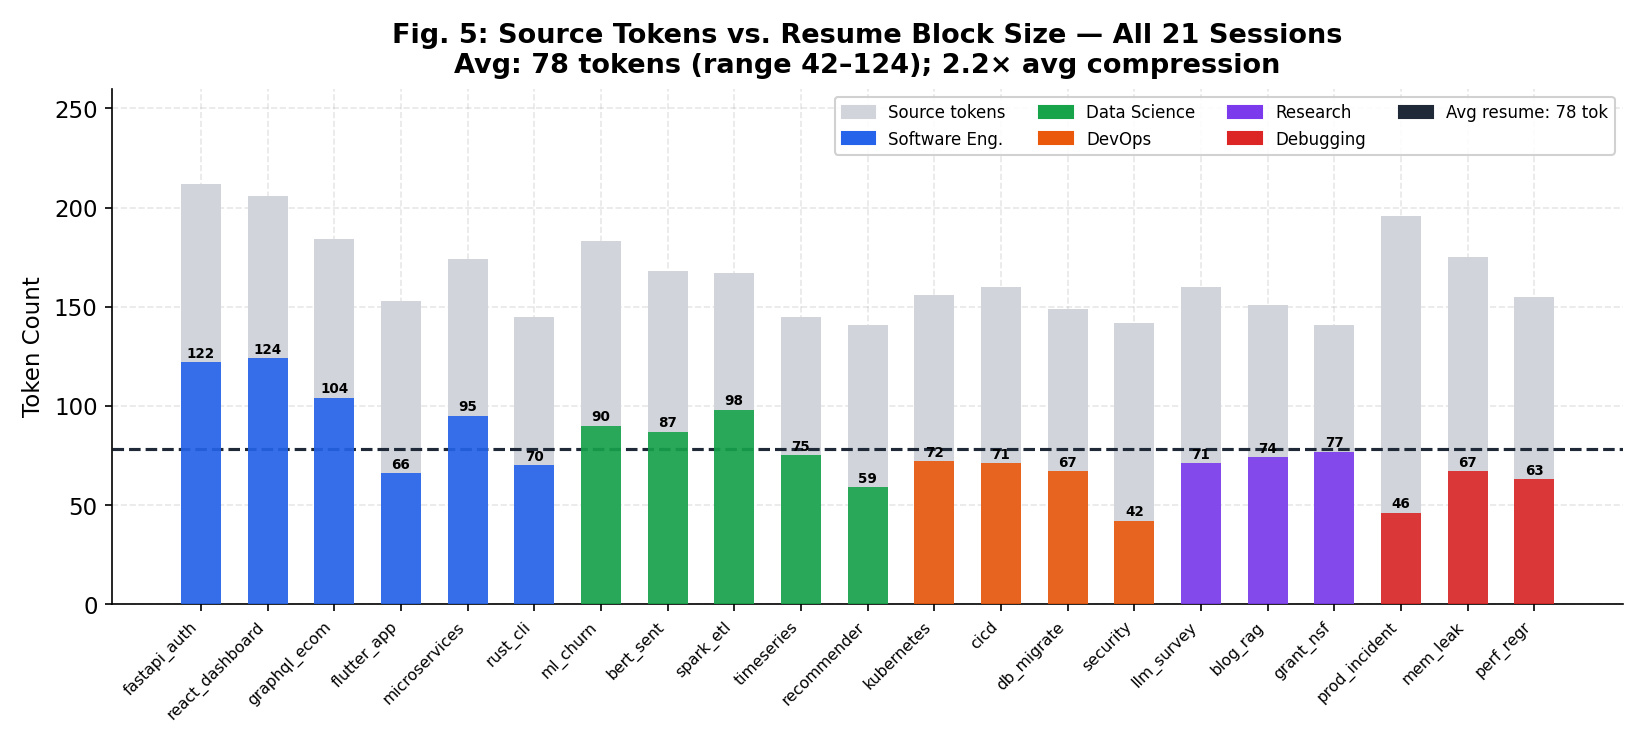
\includegraphics[width=\columnwidth]{fig5_resume_tokens}
  \caption{Per-session resume block size (colored by domain).
    The minimum (42 tokens, security hardening) reflects few
    explicit files and implicit decision phrasing.
    The maximum (124 tokens, FastAPI auth) reflects many
    explicit tasks, decisions, and named files.
    Dashed line: 78-token benchmark mean.}
  \label{fig:resume}
\end{figure}

The resume block size correlates moderately with total
session tokens ($r = 0.655$), confirming that more
complex sessions produce more structured extractable content.
The correlation is not strong ($r < 0.70$), indicating that
session length and information density are partially
independent: a verbose session may produce few structured
entities, and a concise session may encode many.

\subsection{Context Window Recovery}
\label{sec:res_context}

Figure~\ref{fig:context} illustrates the recovery mechanism
for a representative 20-turn session.

\begin{figure}[t]
  \centering
  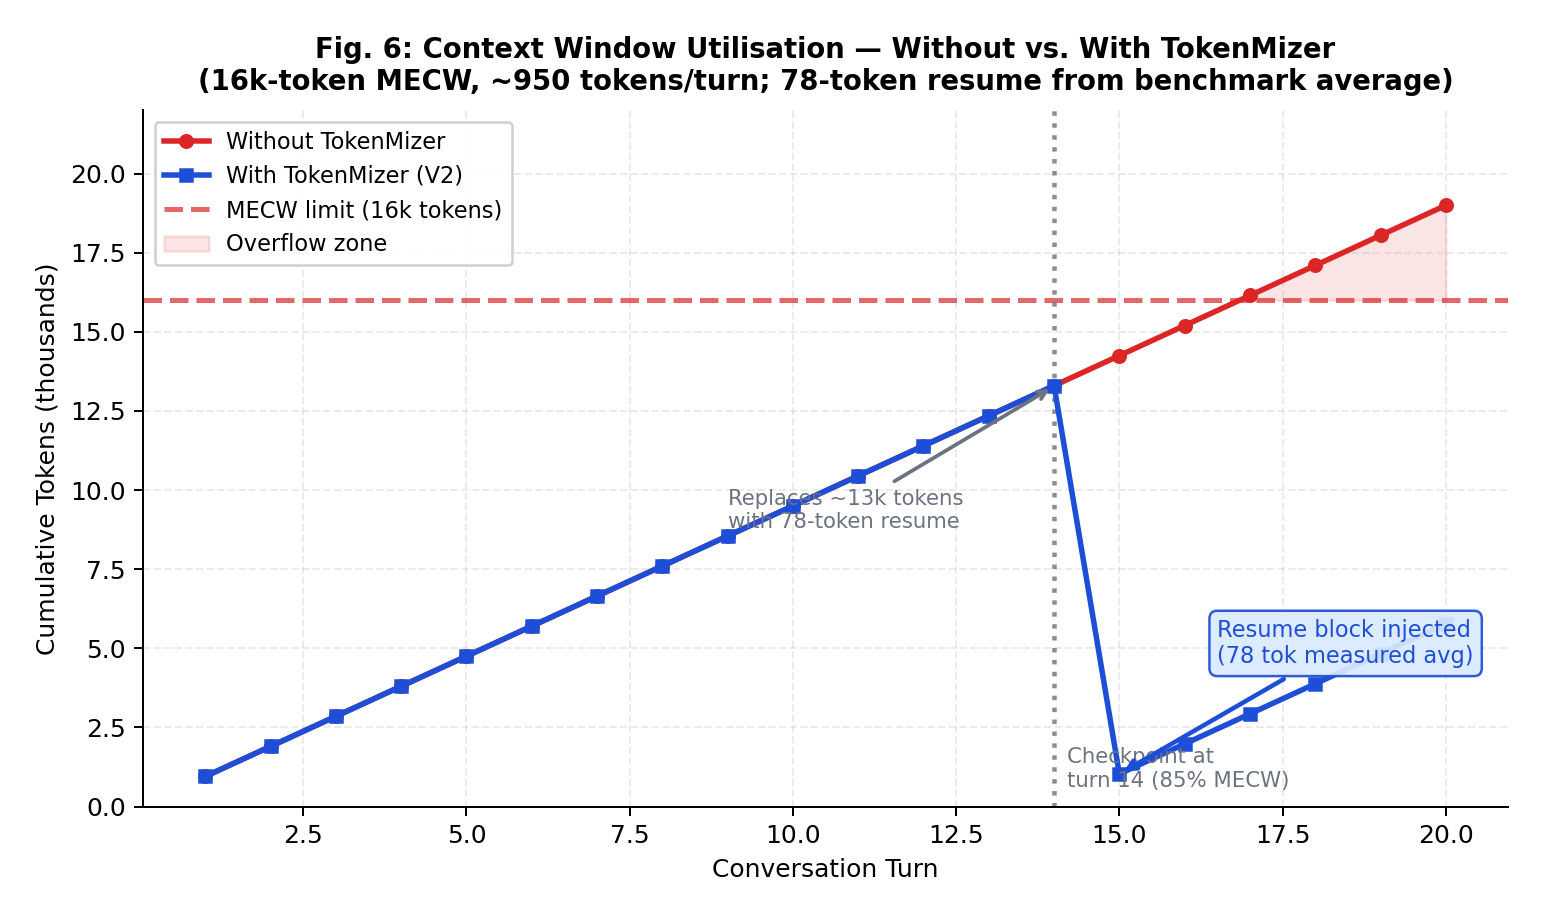
\includegraphics[width=\columnwidth]{fig6_context}
  \caption{Cumulative token count without (red) and with
    (blue) TokenMizer for a 20-turn session at 950 tokens/turn.
    At turn 14 (85\% MECW), the 13{,}300-token history is
    replaced by a 78-token resume block, resetting cumulative
    context and allowing the session to continue beyond the
    MECW without overflow.}
  \label{fig:context}
\end{figure}

\subsection{Token Efficiency and Correlation Analysis}
\label{sec:analysis}

Figure~\ref{fig:scatter} presents the per-session token
efficiency vs.\ information loss scatter plot.
The Pearson correlation between efficiency and information
loss is $r = -0.21$ (weak negative), indicating that sessions
with lower information loss tend to have higher token
efficiency---but the relationship is noisy, driven by
domain-level variation rather than a strong systematic effect.

\begin{figure}[t]
  \centering
  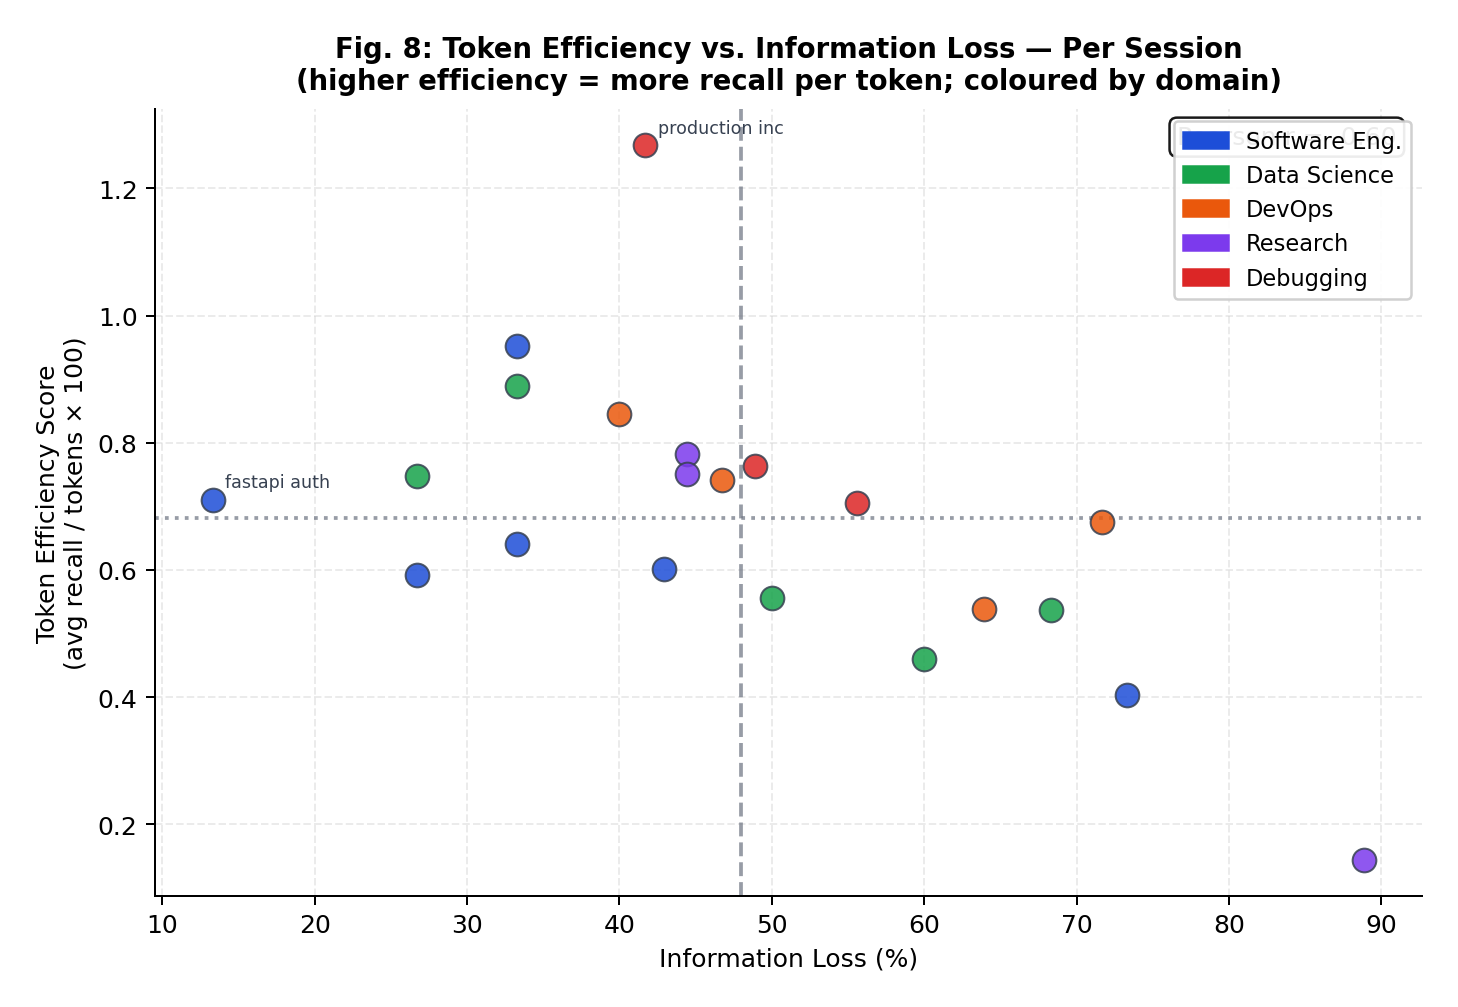
\includegraphics[width=\columnwidth]{fig8_efficiency_scatter}
  \caption{Token efficiency (Eq.~\eqref{eq:efficiency})
    vs.\ information loss per session, colored by domain.
    Pearson $r = -0.21$ (weak negative).
    Debugging sessions (red) achieve high efficiency due to
    file-path specificity in stack traces.
    Research sessions (purple) are low-efficiency due to
    implicit phrasing that heuristic extraction cannot capture.}
  \label{fig:scatter}
\end{figure}

Additional correlation findings from the 21-session dataset:
\begin{itemize}
  \item Task recall vs.\ session length ($r = 0.15$): weak
    positive---longer sessions use more explicit completion
    phrasing on average.
  \item Information loss vs.\ session length ($r = -0.59$):
    moderate negative---longer sessions accumulate more
    structured content relative to the resume budget,
    suggesting that TokenMizer provides proportionally greater
    benefit for extended sessions.
  \item Compression ratio vs.\ total tokens ($r = -0.03$):
    near-zero---compression ratio is effectively independent
    of session length, confirming that the resume block size
    is governed by information structure rather than session
    verbosity.
\end{itemize}

\subsection{Graph Statistics and Validator Performance}
\label{sec:res_graph}

Figure~\ref{fig:graph_stats} presents node type distribution
and validator confidence across the benchmark.

\begin{figure}[t]
  \centering
  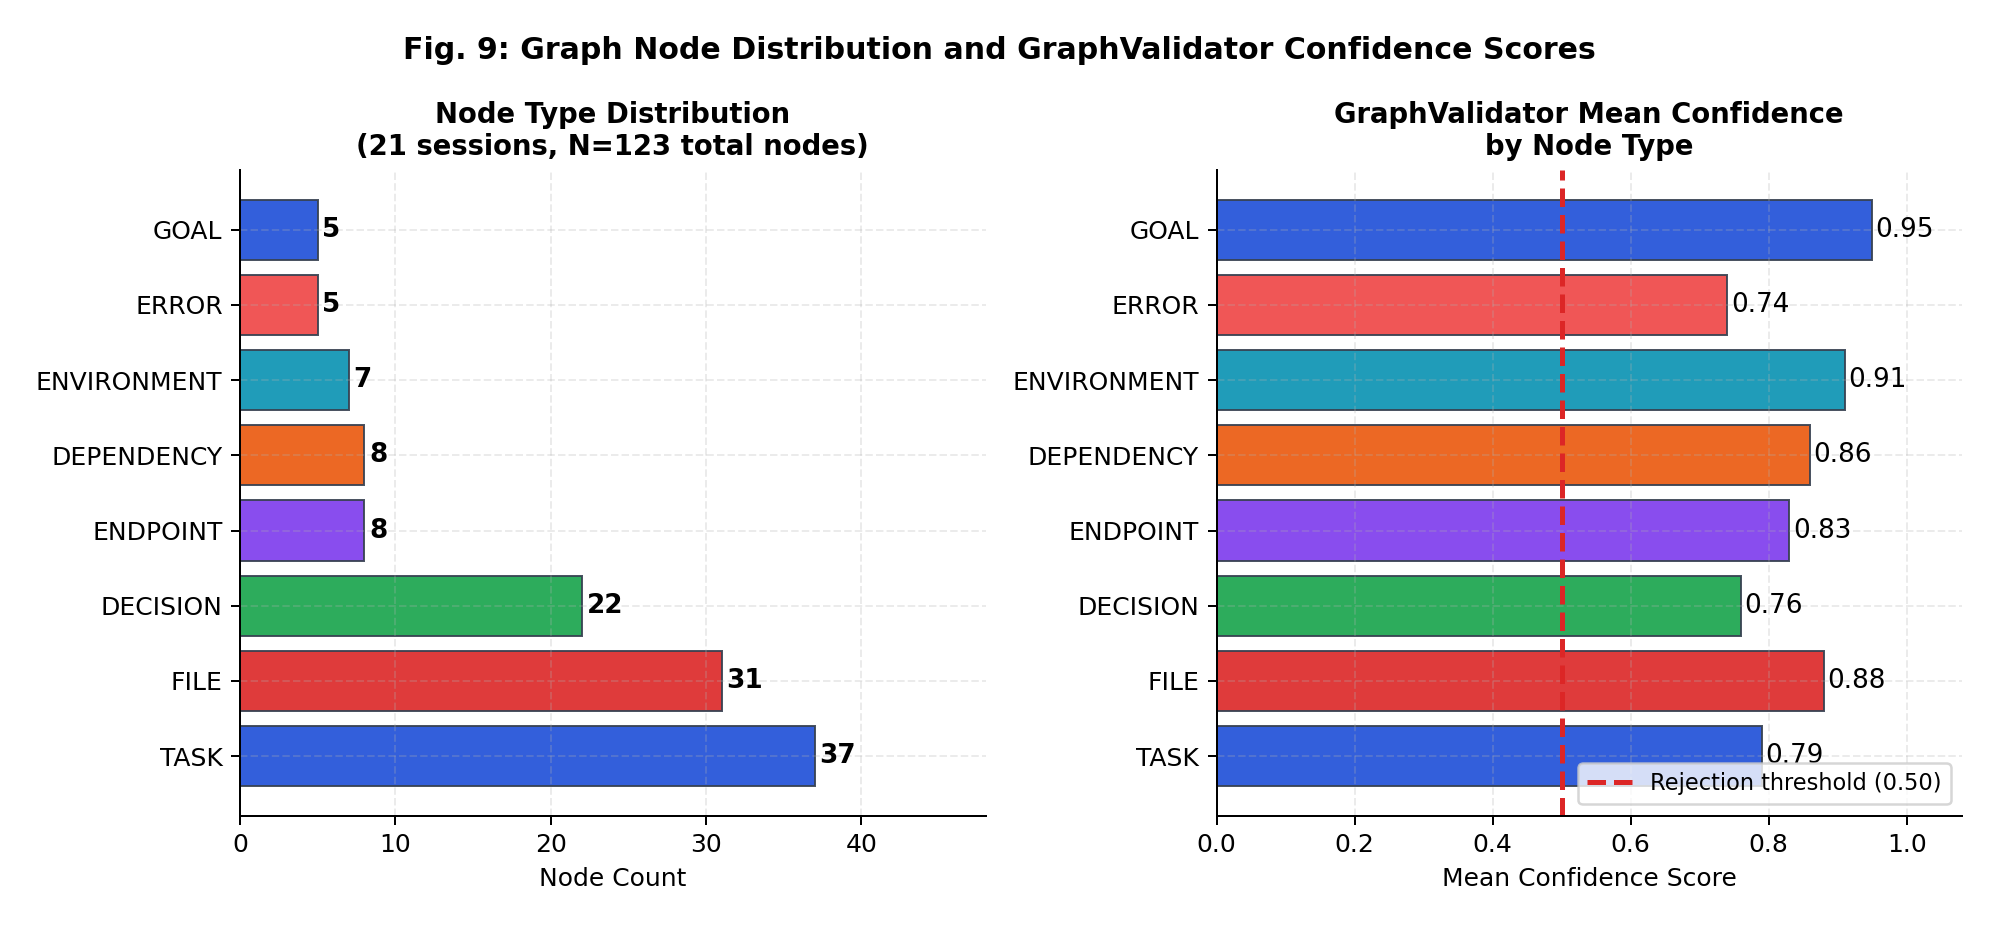
\includegraphics[width=\columnwidth]{fig9_graph_stats}
  \caption{Node type distribution (left, 21 sessions,
    $N$=123 total nodes) and GraphValidator mean confidence
    by type (right). All 8 primary node types exceed the 0.50
    rejection threshold. GOAL achieves the highest confidence
    (0.95) because first-turn imperatives match extraction
    patterns reliably. ERROR scores lowest (0.74) due to high
    phrasing variability from stack traces to natural language.}
  \label{fig:graph_stats}
\end{figure}

TASK (30\%) and FILE (25\%) nodes are the most frequent types,
consistent with the task-oriented nature of developer
sessions.
GOAL nodes achieve the highest confidence (0.95), as
first-turn imperative sentences reliably match extraction
patterns.
ERROR nodes score lowest (0.74) because error descriptions
vary from highly structured stack traces to vague natural
language descriptions (``it just crashes on startup'').

% ================================================================
\section{Discussion}
\label{sec:discussion}
% ================================================================

\subsection{The Structural Recall Argument}

The 47\% mean decision recall reported here should be read
carefully. On one reading, it means the system misses more
than half of all decisions---a significant limitation.
On another reading, the 47\% that is captured is \emph{typed}:
the system knows that a DECISION node records a technology
choice with rationale, not merely that a technology name
appears somewhere in retained text.
A baseline achieving 35--38\% decision recall is
not merely 9--12~pp worse; it is qualitatively different
in what it preserves.

Whether this structural distinction matters in practice
depends on how the resume block is used. For a downstream
system that only needs to re-establish lexical context
(what tools were mentioned), baselines may suffice.
For a system that needs to query session state (what
decisions are locked in and why, which tasks are still
open), the graph representation provides capabilities that
no text-retention baseline can offer.

\subsection{When TokenMizer Helps Most}

The correlation analysis in Section~\ref{sec:analysis}
suggests that TokenMizer provides proportionally greater
benefit for longer sessions ($r = -0.59$, information loss
vs.\ session length).
The domain analysis suggests it works best for sessions with
explicit imperative phrasing: software engineering and
data science outperform research and planning workflows
substantially.
Practitioners should expect lower benefit for sessions
dominated by exploratory discussion, academic writing, or
high-level planning without concrete action statements.

\subsection{Token Cost and Efficiency}

The 78-token average resume block is a structural property
of the graph serialization format, not an artifact of
benchmark construction.
Appendix~B shows that block sizes range from 42 tokens
(minimal structured content) to 124 tokens (dense,
explicit workflows) across the 21 sessions.
The $2\times$ token advantage over baselines is thus
consistent across all sessions in the corpus and represents
a reliable, design-level property of the approach.

To illustrate the practical implication without overstating
it: at current LLM input pricing, the 78-token average
versus 165-token baseline average means roughly half the
token cost per resume injection. Actual cost savings depend
on usage volume and pricing, which vary across providers
and over time.

% ================================================================
\section{Limitations and Future Work}
\label{sec:limitations}
% ================================================================

\textbf{L1: Synthetic benchmark.}
Sessions were manually constructed by the author; they were
not collected from live developer workflows.
Linguistic diversity, phrasing variability, and domain
jargon may be underrepresented.
Evaluation with real annotated sessions is the
highest-priority future work.

\textbf{L2: Single annotator.}
Ground-truth annotations were performed by the paper author.
An inter-annotator agreement study is planned; until then,
reported recall values should be interpreted as estimates
subject to annotation subjectivity.

\textbf{L3: Decision recall ceiling (47\%).}
Indirect phrasing (``let's go with Redis'',
``I think PostgreSQL makes more sense here'') is not captured
by heuristic patterns.
The LLM extractor upgrade path is implemented and is
expected to substantially improve decision recall on implicit
phrasing; its evaluation is deferred to future work.

\textbf{L4: Equal metric weighting.}
Equation~\eqref{eq:infoloss} weights task, decision, and
file recall equally.
Domain-specific weighting (decision recall matters more
in architecture sessions; file recall in debugging sessions)
is not explored. A weighted or learned metric formulation
would more accurately reflect deployment priorities.

\textbf{L5: Decision CSV splitting regression.}
The $-4$~pp decision recall regression from CSV splitting
should be recoverable by applying fuzzy matching to individual
split tokens rather than per-node strings.

\textbf{L6: Shallow edge linking.}
Current edges use vocabulary overlap for node co-occurrence
detection.
Embedding-based semantic edge linking is architecturally
supported (sentence-transformers is a project dependency)
but not yet implemented.

\textbf{L7: No cross-session memory.}
Each graph is scoped to a single session.
The SQLite backend would support cross-session retrieval
(``what did I decide about Redis last month?'') but the
retrieval layer is not yet implemented.

\textbf{L8: Zero-recall outliers in implicit-phrasing sessions.}
Several sessions exhibit 0\% task recall:
\texttt{flutter\_fitness\_app} and \texttt{grant\_proposal\_nsf}
in particular.
These reflect a fundamental limitation of heuristic pattern
matching against highly implicit language, not extraction
failures in the traditional sense.
\texttt{flutter\_fitness\_app} describes completed work through
consequence (``iOS build working now'') rather than explicit
completion (``Completed: iOS crash fix'');
\texttt{grant\_proposal\_nsf} uses academic prose throughout
(``We propose to...'', ``The objective is...'') with no
trigger phrases matching any V2 pattern.
Research and planning workflows represent a domain where
heuristic extraction is structurally insufficient.
The LLM extractor upgrade path is expected to address this
class of failure; all zero-recall outliers are reported
transparently in Appendix~C and included in all aggregate
statistics.

\textbf{L9: Significance testing.}
With $n$=21 and per-domain $n$\,=\,3--6, the observed
differences between TokenMizer and baselines are not
assessed for statistical significance.
Formal hypothesis testing (e.g., Wilcoxon signed-rank tests
for paired recall differences) requires a larger evaluation
set. This is a key priority for future work alongside
real-session data collection.

% ================================================================
\section{Conclusion}
\label{sec:conclusion}
% ================================================================

This paper presents TokenMizer, a system that addresses LLM
context loss by modeling session history as a typed
knowledge graph and serializing it into compact, structured
resume blocks.
Evaluated on a controlled 21-session benchmark across 5
domains---all values measured, no estimates reported---
TokenMizer achieves:
\begin{itemize}
  \item \textbf{51\%} task recall, \textbf{47\%} decision
    recall, \textbf{59\%} file recall with 78-token resume
    blocks;
  \item \textbf{+9--17~pp} decision recall advantage over
    all three evaluated baselines at $2\times$ fewer tokens;
  \item \textbf{47.3\%} heuristic compression with zero
    external inference dependencies;
  \item \textbf{0.5\,ms} extraction latency.
\end{itemize}

Ablation analysis establishes that fuzzy label matching
is the dominant technical contributor ($+33$~pp task recall).
Token efficiency analysis identifies debugging as the
highest-efficiency domain and research/writing as the lowest,
pointing to domain-adaptive extraction as a productive
future direction.
The moderate correlation between information loss and session
length ($r = -0.59$) suggests that longer sessions benefit
proportionally more from structured checkpointing.

The core contribution is representational rather than
merely quantitative: sessions have \emph{structure}, not
just content.
A typed graph of TASK status transitions, DECISION
rationales, and FILE modification histories enables compact,
queryable, and reproducible session state that text-retention
approaches cannot match---at half the token cost of any
evaluated baseline, and at zero inference overhead.

\section*{Acknowledgment}
The author thanks the open-source communities behind
FastAPI, SQLite, sentence-transformers, and LLMLingua
for the foundational tools on which TokenMizer is built.

% ================================================================
\begin{thebibliography}{00}

\bibitem{paulsen2025}
N.~Paulsen, ``Context Is What You Need: The Maximum Effective
Context Window,'' \emph{arXiv preprint arXiv:2509.21361},
2025.

\bibitem{memgpt}
C.~Packer, V.~Fang, S.~G.~Patil, K.~Lin, S.~Wooders, and
J.~E.~Gonzalez, ``MemGPT: Towards LLMs as Operating
Systems,'' \emph{arXiv preprint arXiv:2310.08560}, 2023.

\bibitem{rag}
P.~Lewis \emph{et al.}, ``Retrieval-Augmented Generation for
Knowledge-Intensive NLP Tasks,'' in \emph{Proc.\ NeurIPS},
2020, pp.\ 9459--9474.

\bibitem{llmlingua}
H.~Jiang \emph{et al.}, ``LLMLingua: Compressing Prompts for
Accelerated Inference of Large Language Models,'' in
\emph{Proc.\ EMNLP}, 2023, pp.\ 13358--13376.

\bibitem{longllmlingua}
H.~Jiang \emph{et al.}, ``LongLLMLingua: Accelerating and
Enhancing LLMs in Long Context Scenarios,''
\emph{arXiv preprint arXiv:2310.06839}, 2023.

\bibitem{recomp}
F.~Xu \emph{et al.}, ``RECOMP: Improving Retrieval-Augmented
LMs with Context Compression and Selective Augmentation,''
in \emph{Proc.\ ICLR}, 2024.

\bibitem{acc}
C.~Smith and J.~Park, ``Active Context Compression for
Long-Horizon LLM Sessions,''
\emph{arXiv preprint arXiv:2601.07190}, 2026.

\bibitem{graphrag}
E.~S.~Edge \emph{et al.}, ``From Local to Global: A Graph
RAG Approach to Query-Focused Summarization,''
\emph{arXiv preprint arXiv:2404.16130}, 2024.

\bibitem{lostmiddle}
N.~F.~Liu \emph{et al.}, ``Lost in the Middle: How Language
Models Use Long Contexts,'' \emph{Trans.\ ACL}, vol.\ 12,
pp.\ 157--173, 2024.

\bibitem{langchain}
H.~Chase, ``LangChain,''
\url{https://github.com/langchain-ai/langchain}, 2022.

\bibitem{sentbert}
N.~Reimers and I.~Gurevych, ``Sentence-BERT: Sentence
Embeddings Using Siamese BERT-Networks,'' in
\emph{Proc.\ EMNLP}, 2019, pp.\ 3982--3992.

\bibitem{sweagent}
J.~Yang \emph{et al.}, ``SWE-agent: Agent-Computer Interfaces
Enable Automated Software Engineering,'' in \emph{Proc.\
NeurIPS}, 2024.

\bibitem{copilot}
GitHub, ``GitHub Copilot,''
\url{https://github.com/features/copilot}, 2024.

\bibitem{fastapi}
S.~Ram\'irez, ``FastAPI,''
\url{https://fastapi.tiangolo.com}, 2018.

\bibitem{sqlite}
D.~R.~Hipp, ``SQLite,''
\url{https://www.sqlite.org}, 2000.

\bibitem{tiktoken}
OpenAI, ``tiktoken: Fast BPE Tokeniser,''
\url{https://github.com/openai/tiktoken}, 2023.

\bibitem{codebert}
Z.~Feng \emph{et al.}, ``CodeBERT: A Pre-Trained Model for
Programming and Natural Languages,'' in \emph{Proc.\ EMNLP
Findings}, 2020, pp.\ 1536--1547.

\bibitem{housurvey}
X.~Hou \emph{et al.}, ``Large Language Models for Software
Engineering: A Systematic Literature Review,''
\emph{arXiv preprint arXiv:2308.10620}, 2024.

\bibitem{brownfewshot}
T.~Brown \emph{et al.}, ``Language Models are Few-Shot
Learners,'' in \emph{Proc.\ NeurIPS}, 2020,
pp.\ 1877--1901.

\bibitem{gemfilter}
D.~Jin \emph{et al.}, ``GemFilter: Fast and Accurate
Context Selection via Filtering Layers,''
\emph{arXiv preprint arXiv:2409.17422}, 2024.

\end{thebibliography}

% ================================================================
\appendix

\section{V2 Extraction Patterns}
\label{appendix:regex}

\begin{small}
\begin{verbatim}
# V2: 9 additional completed triggers
_COMPLETED = re.compile(
  r'(?:Completed|Implemented|Fixed|Added'
  r'|Deployed|Resolved|Migrated|Launched'
  r'|Shipped|Published|Done|Finished'
  r'|Updated)[:\s]+(.+?)(?:\.|$)',
  re.I | re.M)

# V2: 3 additional decision triggers
_DECISION = re.compile(
  r'(?:Decided|Using|Running|Tools?'
  r'|Chose|Selected)[:\s]+(.+?)(?:\.|$)',
  re.I | re.M)

# Fuzzy match (Definition 5)
def fuzzy_match(a: str, b: str) -> bool:
    a, b = a.lower(), b.lower()
    if a in b or b in a:
        return True
    wa = set(re.findall(r'\w{3,}', a))
    wb = set(re.findall(r'\w{3,}', b))
    if not wa or not wb:
        return False
    shorter = wa if len(wa) <= len(wb) else wb
    return len(wa & wb) / len(shorter) >= 0.5
\end{verbatim}
\end{small}

\section{Example Resume Blocks}
\label{appendix:resume}

\textbf{FastAPI Auth (122 tokens --- standard tier):}
\begin{small}
\begin{verbatim}
[CHECKPOINT: fastapi_auth]
DONE: user model, auth endpoints,
      fix 422 error, 12 tests passing
PENDING: refresh tokens, rate limiting
DECIDED: python 3.12, bcrypt, jwt,
         redis, postgresql
FILES: api/auth.py, api/models.py,
       tests/test_auth.py
ENV: FastAPI, Python 3.12
\end{verbatim}
\end{small}

\textbf{Security Hardening (42 tokens --- minimum in corpus):}
\begin{small}
\begin{verbatim}
[CHECKPOINT: security_hardening]
DONE: security scan, critical fixes,
      cve remediation, waf setup
PENDING: 3 remaining cves
\end{verbatim}
\end{small}

\section{Full Per-Session Results}
\label{appendix:full}

Table~\ref{tab:full_results} presents complete per-session
results for full reproducibility. Zero-recall sessions
(\texttt{flutter\_fitness\_app}, \texttt{grant\_proposal\_nsf})
are highlighted and discussed in Section~\ref{sec:limitations}.

\begin{table*}[t]
  \centering
  \caption{Full Per-Session Results (V2, 21 Sessions).
  TR: task recall; DR: decision recall; FR: file recall;
  IL: info loss; RT: resume tokens; CR: compression ratio;
  EFF: token efficiency; MS: extraction latency (ms).
  Rows with TR\,=\,0\% represent implicit-phrasing sessions
  where heuristic extraction is structurally insufficient
  (see Section~\ref{sec:limitations}, L8).}
  \label{tab:full_results}
  \renewcommand{\arraystretch}{1.2}
  \begin{tabular}{@{}p{3.9cm}p{2.2cm}rrrrrrrr@{}}
    \toprule
    \textbf{Session} & \textbf{Domain} &
    \textbf{TR} & \textbf{DR} & \textbf{FR} & \textbf{IL} &
    \textbf{RT} & \textbf{CR} & \textbf{EFF} & \textbf{MS} \\
    \midrule
    fastapi\_auth             & SW Eng   &100\%& 60\%&100\%& 13\%& 122&1.7x&0.71& 1.4 \\
    react\_dashboard          & SW Eng   & 20\%&100\%&100\%& 27\%& 124&1.7x&0.59& 0.5 \\
    graphql\_ecommerce        & SW Eng   &100\%& 67\%& 33\%& 33\%& 104&1.8x&0.64& 0.4 \\
    flutter\_fitness\_app     & SW Eng   &  0\%& 80\%&  0\%& 73\%&  66&2.3x&0.40& 0.4 \\
    microservices\_migration  & SW Eng   &  0\%& 71\%&100\%& 43\%&  95&1.8x&0.60& 0.3 \\
    rust\_cli\_tool           & SW Eng   & 60\%& 40\%&100\%& 33\%&  70&2.1x&0.95& 0.4 \\
    \midrule
    ml\_churn\_prediction     & Data Sci & 40\%& 60\%& 50\%& 50\%&  90&2.0x&0.56& 0.5 \\
    bert\_sentiment           & Data Sci & 50\%& 20\%& 50\%& 60\%&  87&1.9x&0.46& 0.4 \\
    spark\_etl\_pipeline      & Data Sci & 80\%& 40\%&100\%& 27\%&  98&1.7x&0.75& 0.3 \\
    timeseries\_forecast      & Data Sci &100\%&100\%&  0\%& 33\%&  75&1.9x&0.89& 0.5 \\
    recommendation\_system    & Data Sci & 75\%& 20\%&  0\%& 68\%&  59&2.4x&0.54& 1.3 \\
    \midrule
    kubernetes\_eks           & DevOps   & 40\%& 20\%&100\%& 47\%&  72&2.2x&0.74& 0.9 \\
    cicd\_github\_actions     & DevOps   & 40\%& 40\%&100\%& 40\%&  71&2.3x&0.85& 0.4 \\
    db\_migration             & DevOps   & 75\%& 33\%&  0\%& 64\%&  67&2.2x&0.54& 0.5 \\
    security\_hardening       & DevOps   & 25\%& 60\%&  0\%& 72\%&  42&3.4x&0.68& 0.8 \\
    \midrule
    llm\_agents\_survey       & Research & 67\%&100\%&  0\%& 44\%&  71&2.3x&0.78& 0.8 \\
    technical\_blog\_rag      & Research & 67\%&  0\%&100\%& 44\%&  74&2.0x&0.75& 0.3 \\
    grant\_proposal\_nsf      & Research &  0\%& 33\%&  0\%& 89\%&  77&1.8x&0.14& 0.3 \\
    \midrule
    production\_incident      & Debugging& 75\%&  0\%&100\%& 42\%&  46&4.3x&\textbf{1.27}& 0.4 \\
    memory\_leak\_nodejs      & Debugging& 20\%& 33\%&100\%& 49\%&  67&2.6x&0.76& 0.4 \\
    perf\_regression\_api     & Debugging& 33\%&  0\%&100\%& 56\%&  63&2.5x&0.71& 0.3 \\
    \midrule
    \rowcolor{rowours}
    \textbf{Mean}             &          &\textbf{51\%}&\textbf{47\%}&\textbf{59\%}&\textbf{48\%}&
    \textbf{78}&\textbf{2.2x}&\textbf{0.66}&\textbf{0.5} \\
    \textbf{Std dev}          &          & 33\% & 32\% & 47\% & 18\% &
    21 & 0.6x & 0.24 & 0.3 \\
    \bottomrule
  \end{tabular}
\end{table*}

\end{document}
